\let\primyear\year
\documentclass{ieeeaccess}
\let\accyear\year\let\year\primyear
\usepackage{tikz}
\let\year\accyear
\definecolor{accessblue}{cmyk}{1,.43,0,.09}% PANTONE 3015C process equivalent (spot colour breaks with pgf)
\usepackage{mciteplus}
\def\xfigwd{0pt}
\usepackage[utf8]{inputenc}
\usepackage{microtype}
\usepackage{amsmath,amssymb}
\usepackage{graphicx}
\usepackage{booktabs}
\usepackage{multirow}
\usepackage{array}
\usepackage{tabularx}
\usepackage[table]{xcolor}
\usetikzlibrary{positioning,arrows.meta,fit,calc,backgrounds,shapes.geometric}
\usepackage{algorithm}
\usepackage[noend]{algpseudocode}
\usepackage{enumitem}
\setlist{nosep,leftmargin=*}
\usepackage[hidelinks]{hyperref}
\usepackage[capitalise,nameinlink]{cleveref}
\crefname{algorithm}{Algorithm}{Algorithms}
\crefname{equation}{Eq.}{Eqs.}
\crefname{line}{line}{lines}

\definecolor{ink}{HTML}{0B0B0B}
\definecolor{muted}{HTML}{52514E}
\definecolor{band}{HTML}{F0EFEC}
\definecolor{accent}{HTML}{2A78D6}
\definecolor{warm}{HTML}{EB6834}
\newcommand{\ci}[2]{\scriptsize[#1, #2]}
\algrenewcommand\algorithmicrequire{\textbf{Input:}}
\algrenewcommand\algorithmicensure{\textbf{Output:}}
\algnewcommand{\LineComment}[1]{\State \textcolor{muted}{\(\triangleright\) #1}}
\DeclareMathOperator*{\topk}{top\text{-}k}
\DeclareMathOperator{\AUC}{AUC}
\DeclareMathOperator{\BCE}{BCE}
\DeclareMathOperator{\GAP}{GAP}

\renewcommand{\topfraction}{0.9}
\renewcommand{\bottomfraction}{0.8}
\renewcommand{\textfraction}{0.07}
\renewcommand{\floatpagefraction}{0.75}
\setcounter{topnumber}{3}
\setcounter{totalnumber}{5}


\begin{document}
\history{Date of publication xxxx 00, 0000, date of current version xxxx 00, 0000.}
\doi{10.1109/ACCESS.2026.DOI}

\title{Adversarial Deconfounding With Pseudo Device Labels Does Not Reduce Device-Associated Bias in Pneumothorax Detection: A Pre-Registered, Multi-Seed External Evaluation of Twelve Models}
\author{\uppercase{Mohanad Dawood Salman}\authorrefmark{1}, \uppercase{Luay Ibrahim Khalaf}\authorrefmark{1}, \uppercase{Omar Ahmed Razooqi}\authorrefmark{2}, and \uppercase{Salwa Khalid Abdulateef}\authorrefmark{1}}
\address[1]{Computer Science Department, College of Computer Science and Mathematics, Tikrit University, Tikrit, Salah al-Deen 34001, Iraq}
\address[2]{Department of Hadith and Its Sciences, College of Islamic Sciences, Tikrit University, Tikrit, Salah al-Deen 34001, Iraq}
\tfootnote{This research did not receive any specific grant from funding agencies in the public, commercial, or not-for-profit sectors.}

\markboth
{Salman \headeretal: Adversarial Deconfounding Does Not Reduce Device-Associated Bias in Pneumothorax Detection}
{Salman \headeretal: Adversarial Deconfounding Does Not Reduce Device-Associated Bias in Pneumothorax Detection}

\corresp{Corresponding author: Salwa Khalid Abdulateef (e-mail: khalid.salwa@tu.edu.iq).}

\begin{abstract}
Pneumothorax classifiers trained on public chest radiographs can associate the disease label with visible devices, particularly chest drains. Under a protocol registered in a version-controlled repository before external testing, we tested whether a segmentation-based detector trained with a gradient-reversal adversary against device pseudo-labels detects pneumothorax without visible devices better on external data. Twelve configurations (54 training runs), including Group DRO and a radiology foundation model, were developed on SIIM-ACR and evaluated once on the NIH device cohort (classification) and PTX-498 (positives only). The proposed model did not outperform the baselines on either primary endpoint: its device-absent sensitivity (0.22) was two cases below the best baseline (95\% CI of the difference $-$0.14 to 0.00), and its device-minus-device-absent AUROC gap was the largest point estimate (0.26; 95\% CI 0.15--0.37 over patients and 0.12--0.43 over patients and training seeds). With training-seed variation included, no pairwise difference was significant after multiplicity adjustment. The adversary reached chance during training, yet device information remained linearly decodable. Positives with chest drains were detected almost perfectly, and among posteroanterior negatives device-bearing images scored higher in all configurations (significantly in eight). The pseudo-label captured 98\% of annotated drains but was much broader than drains, and patient overlap between ChestX-ray14-derived datasets inflated device-present performance; 19 device-absent positives remained after its removal. The negative result concerns this implementation with a broad device proxy. Device-stratified external metrics, seed-level uncertainty and patient-level independence checks should be reported routinely.
\end{abstract}

\begin{keywords}
Chest radiography, deep learning, domain-adversarial training, external validation, medical image segmentation, negative result, pneumothorax, pre-registration, shortcut learning.
\end{keywords}

\titlepgskip=-21pt

\maketitle

%% ============================================================ INTRODUCTION
\section{Introduction}
\label{sec:intro}

Deep learning systems for chest radiographs often exploit features that correlate with a label in the training data but are not the pathology itself \cite{geirhos2020shortcut,zech2018variable,degrave2021covid,badgeley2019hip,banerjee2023shortcuts}. In pneumothorax detection, many radiographs labelled positive in public datasets were acquired after treatment and therefore show a chest drain. A model can reach a high overall AUROC by responding to the drain and still perform poorly on radiographs without a drain, which include those of patients whose pneumothorax has not yet been recognised and treated \cite{oakdenrayner2020hidden,taylor2018pneumothorax,rueckel2020tubes}. Pooled estimates suggest that pneumothorax detectors match physicians \cite{sugibayashi2023meta,katzman2024meta}, but most primary studies carry a high risk of bias and few report performance stratified by the presence of devices.

Two families of methods are commonly used to reduce such shortcuts. Domain-adversarial training removes information about a nuisance attribute from the representation by gradient reversal \cite{ganin2015dann,kim2019learning,zhao2020confounder}. Group distributionally robust optimisation (Group DRO) up-weights the worst-performing group defined by label and attribute \cite{sagawa2020groupdro}. A third, architectural idea is to derive the image-level score from the segmentation of the air itself, so that evidence outside the pneumothorax region cannot drive the decision \cite{rueckel2021annotations}.

This study tested whether combining these ideas yields a better detector of pneumothorax on radiographs without visible devices (``device-absent'' pneumothorax) on external data. To avoid the analytic flexibility that inflates positive results, all endpoints, pass thresholds, baselines, ablations and statistical tests were registered in the version-controlled code repository and frozen before any external test set was opened \cite{nosek2018prereg} (\cref{sec:design}). The original design relied on CANDID-PTX \cite{feng2021candid}, the only public dataset we know of with chest-tube segmentation masks. Access could not be obtained; the dataset is reported to be unavailable outside Health New Zealand since February 2024. We therefore executed a pre-registered amendment (``Plan B'') that uses pseudo-labelled visible devices in place of chest tubes.

The hypothesis was not supported. The study is reported in full because (i) it is informative for anyone applying adversarial deconfounding with proxy labels, (ii) the same experiment provides a controlled, multi-seed audit of device-associated differences across twelve models, including a radiology foundation model \cite{perezgarcia2025raddino}, and (iii) it documents a failure of threshold transfer between two public pneumothorax datasets.

The design choices follow from the problem. Gradient reversal \cite{ganin2015dann} was chosen because it is the most widely used representation-level method for removing a known nuisance attribute and needs only an attribute label, not a mask. Top-$k$ mask pooling was chosen because it ties the image-level score to the pixels that the network segments as pneumothorax, which, if the segmentation is anatomically correct, should exclude device evidence elsewhere in the image. Pseudo-labels were used because no accessible dataset provides chest-tube labels for the development images. The study differs from earlier work in four respects. Previous studies either measured the drain shortcut without mitigating it \cite{jimenez2023shortcuts,sourget2025clip,li2025featurequality} or proposed a mitigation and evaluated it against the authors' own baseline \cite{rueckel2021annotations,bandaru2026untreated}; to our knowledge none pre-registered the comparison or reported device-stratified external results across several re-trained alternatives. Here a mitigation was specified, pre-registered and compared with six re-trained baselines and five variants over 3--5 seeds each, the external test sets were opened once, the device-associated difference was measured in negatives as well as positives, and post hoc analyses examine the proxy label, the decision pathway and the independence of the evaluation directly.

\paragraph{Contributions}
\begin{itemize}
  \item A frozen-before-testing evaluation of an established combination of components (gradient reversal, mask pooling and device pseudo-labels) against six re-trained baselines and five ablation and sensitivity variants (54 training runs), each evaluated once on external data, with a protocol record whose timing is verifiable from the repository host (\cref{sec:design,tab:protocol}). The contribution lies in this evaluation design and its findings, not in a new algorithm.
  \item Evidence that gradient-reversal removal of a pseudo-labelled device attribute, as implemented here, did not reduce the device--device-absent AUROC gap on external data (the largest point estimate of twelve configurations), with patient-cluster and seed-level uncertainty for all endpoints and with training dynamics, probes and an analysis of the top-$k$ decision pixels that explain why (\cref{sec:res-endpoints,sec:res-seeds,sec:res-conv,sec:res-topk}).
  \item A cross-architecture audit showing device-associated differences in every model in the pre-specified analysis (eight of twelve robustly after removal of identified patient overlap), near-perfect detection of drain-bearing positives and device information inside the pneumothorax score of negatives (\cref{sec:res-shortcut,sec:res-strata}).
  \item A quantification of three threats to the validity of evaluations built on public ChestX-ray14-derived data: the breadth of a device proxy relative to chest drains, patient overlap that image-level splitting and near-duplicate removal do not prevent, and score-distribution shift that defeats threshold transfer (\cref{sec:res-pseudo,sec:res-overlap,sec:res-threshold}).
  \item Open code, split files, per-image predictions and all 54 checkpoints.
\end{itemize}

%% ============================================================ RELATED WORK
\section{Related work}
\label{sec:related}

\paragraph{Chest tubes as a confounder in pneumothorax detection}
Rueckel et al.~\cite{rueckel2020tubes} showed on 6{,}434 annotated supine radiographs that thoracic tubes are strong confounders: comparing untreated positives with tube-bearing negatives removed the discriminative power of two public-data algorithms. Rueckel et al.~\cite{rueckel2021annotations} reduced this bias by adding in-image annotations of the visceral pleural line to training. Saliency analyses of vision transformers and CNNs trained on public data revealed a strong bias toward tubes \cite{wollek2023attention}. Jim\'enez-S\'anchez et al.~\cite{jimenez2023shortcuts} released drain annotations for a subset of NIH ChestX-ray14 pneumothorax images and confirmed the shortcut. More recently, Sourget et al.~\cite{sourget2025clip} found that six CLIP-based chest radiograph models all performed worse on pneumothorax without drains, and Li et al.~\cite{li2025featurequality} reported that medical foundation-model encoders, RAD-DINO among them, use chest tubes as a shortcut for pneumothorax classification. The shortcut is not universal. Thian et al.~\cite{thian2021external} found no difference between tube-present and tube-absent radiographs across six external sites, Seah et al.~\cite{seah2021hidden} found a commercial model non-inferior in the intercostal-drain subgroup, and Graf et al.~\cite{graf2020tube} reported comparable performance with and without tubes after lung segmentation and patch classification. Other shortcuts, such as exposure parameters, can also dominate pneumothorax predictions \cite{shu2026exposure}.

\paragraph{Mitigation with attribute labels}
Adversarial and disentanglement methods remove a known confounder from the representation \cite{ganin2015dann,kim2019learning,zhao2020confounder}. In chest radiography they have been used for view position in pneumonia \cite{janizek2020adversarial}, source dataset in COVID-19 \cite{robinson2022disentangle} and race \cite{correa2023cav}. Benchmarks show that such methods help mainly under strong spurious correlation and that latent-space analyses reveal differences that classification metrics miss \cite{muller2026disentangle}. Group DRO optimises the worst group \cite{sagawa2020groupdro}, but reweighting can be problematic when bias is not the only cause of poor performance \cite{kumar2023droinvariant}. For pneumothorax specifically, Bandaru et al.~\cite{bandaru2026untreated} added auxiliary chest-tube detection to improve the classification of untreated pneumothorax.

\paragraph{Mitigation without attribute labels}
When attribute labels are missing, they can be inferred. JTT up-weights examples an initial model misclassifies \cite{liu2021jtt}; pseudo bias-balanced learning predicts per-sample bias labels for chest radiographs \cite{luo2022pbbl}. Worst-group accuracy with inferred groups still trails that with oracle groups, which motivated more precise group inference \cite{han2024gic}. Our design sits between these settings: device labels were inferred by a separately trained classifier, then used as if they were true attribute labels. Counterfactual image editing is a further, data-centric route \cite{cooke2026roentmod}.

\paragraph{Evaluation practice}
Shortcut reliance is often invisible in overall metrics and is more prevalent than reported \cite{unnikrishnan2024pest,vasquez2024cleverhans}. Removing a shortcut in-distribution does not guarantee better behaviour out of distribution \cite{yang2024limits}, and foundation models can encode unwanted attributes \cite{glocker2023foundation}. Saliency maps are an unreliable basis for localisation claims \cite{saporta2022saliency,arun2021saliency}. We therefore rely on stratified external metrics and a score-level device test, and use saliency only as illustration.

\paragraph{Clinical evaluation of pneumothorax detectors}
Clinical studies show that the performance of pneumothorax detectors and of readers assisted by them depends on acquisition conditions. AI assistance improved reader performance most for less experienced readers, and projection type affected performance in the same study \cite{ho2025readers}; a commercial detector was less sensitive on supine radiographs, particularly for small pneumothoraces \cite{nakamura2026supine}; and a detector combined with an electronic notification system shortened the time to treatment \cite{oh2025notification}. These findings motivate reporting performance by projection and by the presence of devices, as done here.

\paragraph{Relation to the closest studies}
Two recent studies are methodologically closest. Bandaru et al.~\cite{bandaru2026untreated} added chest-tube detection as an auxiliary training task, so that the network represents the tube explicitly, and used a separate model to estimate tube labels where they were missing, with the aim of improving the classification of untreated pneumothorax. The present study shares the use of estimated device labels but differs in three respects: the attribute is removed from the pooled representation by gradient reversal rather than predicted as an auxiliary target; the image-level score is computed from the segmentation output by top-$k$ pooling; and an auxiliary device classifier without gradient reversal, after Bandaru et al., is included among the re-trained baselines, so that the two strategies are compared under identical data, splits, training recipe and evaluation. RoentMod \cite{cooke2026roentmod} follows a data-centric route: a text-conditioned image-to-image generative model edits radiographs to add a specified finding while preserving the remaining anatomy, so that the dependence of a classifier on off-target findings can be measured by intervention and reduced by training on counterfactual images. Counterfactual editing tests causal dependence directly, which the stratified comparisons of the present study cannot do; applying it to the removal or insertion of chest drains would require validation of the edited images, which was outside the scope of this study. The present study therefore does not propose a new mitigation algorithm. Its contribution is the evaluation design (a protocol fixed before external testing, twelve re-trained configurations over 3--5 seeds, a single external evaluation, and device-stratified and device-in-score metrics with patient-cluster and seed-level uncertainty) and the findings that this design produces.

\Cref{tab:related} positions this study against the pneumothorax-specific literature.

\begin{table*}[!t]
\centering\scriptsize
\setlength{\tabcolsep}{3pt}
\caption{Pneumothorax studies that examined chest tubes or devices. ``Strat.'' = performance reported by device status; ``Mitig.'' = a method aimed at reducing device reliance. Findings are summarised from the cited abstracts.}
\label{tab:related}
\begin{tabularx}{\linewidth}{@{}p{2.3cm} p{3.1cm} c c X@{}}
\toprule
Study & Data (test) & Strat. & Mitig. & Main finding on devices \\
\midrule
Rueckel et al.~\cite{rueckel2020tubes} & 6{,}434 supine CXRs, single centre & \checkmark & --- & Tubes are strong confounders; untreated vs tube-bearing negatives removes discrimination \\
Rueckel et al.~\cite{rueckel2021annotations} & 3{,}062 supine CXRs & \checkmark & \checkmark & Pleural-line annotations raise AUROC and reduce tube bias \\
Graf et al.~\cite{graf2020tube} & Public benchmark & \checkmark & \checkmark & Lung segmentation + patch classification; comparable with/without tubes \\
Thian et al.~\cite{thian2021external} & Six external sites & \checkmark & --- & No difference with vs without chest tube \\
Seah et al.~\cite{seah2021hidden} & 2{,}557 studies, AU/US & \checkmark & --- & Commercial model non-inferior in drain subgroup \\
Feng et al.~\cite{feng2022triage} & CANDID-PTX & --- & --- & Grad-CAM: negligible confounding reported \\
Jim\'enez-S\'anchez et al.~\cite{jimenez2023shortcuts} & NIH-CXR14 subset & \checkmark & --- & Drain annotations released; shortcut confirmed \\
Wollek et al.~\cite{wollek2023attention} & CXR14, VinBigData, SIIM & --- & --- & Saliency reveals strong tube bias \\
Sourget et al.~\cite{sourget2025clip} & MIMIC, CXR14, NEATX & \checkmark & --- & Six CLIP models worse without drains \\
Li et al.~\cite{li2025featurequality} & Eight foundation encoders & \checkmark & --- & Foundation models use tube shortcut \\
Bandaru et al.~\cite{bandaru2026untreated} & Public data & \checkmark & \checkmark & Auxiliary tube detection for untreated cases \\
\rowcolor{band}\textbf{This study} & NIH device cohort (521), PTX-498 (482) & \checkmark & \checkmark & Pre-registered; 12 models; adversarial debiasing did not reduce the gap; device-associated differences in all models (pre-specified analysis) \\
\bottomrule
\end{tabularx}
\end{table*}

%% ============================================================ METHODS
\section{Materials and methods}
\label{sec:methods}

\subsection{Study design and pre-registration}
\label{sec:design}
The protocol (\texttt{PREREGISTRATION.md} in the code repository) fixed hypotheses, datasets and roles, the operating point, primary and secondary endpoints, ablations, baselines and statistics. Amendment~1 (Plan B) was added on 23 September 2026, before any external evaluation, when CANDID-PTX access proved unavailable. Deviations were recorded on 24 September 2026, again before freezing. The frozen file's SHA-256 hash was written to the repository, and the external-evaluation script refuses to run if the file changes. External test sets were opened once per trained model.

The protocol was registered in the project's version-controlled code repository, not in a public registry such as the Open Science Framework. Commit times are set by the committing computer and are therefore not independent evidence of timing. Independent timestamps are provided by the repository host: GitHub records the time at which each commit is pushed to its servers, and this activity record cannot be edited by repository users. It shows that the protocol draft and Amendment~1 reached the server on 23~September 2026 (11:01 and 17:44~UTC), the recorded deviations and the frozen protocol on 24~September (18:38 and 23:08~UTC), and the first external predictions at 23:24~UTC on 24~September (\cref{tab:protocol}). The repository, including its full history and this record, is public (Data and code availability). In this paper, ``pre-registered'' refers to this repository-based registration. \Cref{fig:design} summarises the design. Reporting follows the spirit of CLAIM and TRIPOD+AI \cite{mongan2020claim,collins2024tripodai}.

\begin{figure*}[!t]
\centering
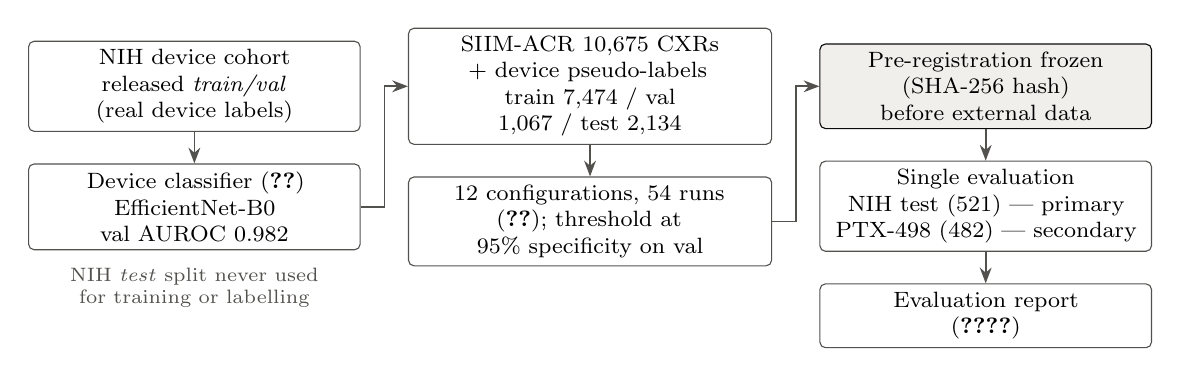
\begin{tikzpicture}[
  node distance=4mm and 6mm,
  box/.style={draw=muted, rounded corners=2pt, align=center, font=\footnotesize, inner sep=3pt, text width=#1},
  box/.default=4.4cm,
  hl/.style={box=#1, fill=band, draw=ink},
  hl/.default=4.4cm,
  arr/.style={-{Stealth[length=2mm]}, draw=muted, line width=0.6pt}]
\node[box=4.0cm] (nihtr) {NIH device cohort\\ released \emph{train/val}\\ (real device labels)};
\node[box=4.0cm, below=of nihtr] (dev) {Device classifier (\cref{alg:pseudo})\\ EfficientNet-B0\\ val AUROC 0.982};
\node[box=4.4cm, right=of nihtr] (siim) {SIIM-ACR 10{,}675 CXRs\\ + device pseudo-labels\\ train 7{,}474 / val 1{,}067 / test 2{,}134};
\node[box=4.4cm, below=of siim] (train) {12 configurations, 54 runs\\ (\cref{alg:train}); threshold at\\ 95\% specificity on val};
\node[hl=4.0cm, right=of siim] (freeze) {Pre-registration frozen\\ (SHA-256 hash)\\ before external data};
\node[box=4.0cm, below=of freeze] (ext) {Single evaluation\\ NIH test (521) --- primary\\ PTX-498 (482) --- secondary};
\node[box=4.0cm, below=of ext] (acc) {Evaluation report\\ (\cref{alg:eval,alg:boot})};
\draw[arr] (nihtr) -- (dev);
\draw[arr] (dev.east) -- ++(3mm,0) |- (siim.west);
\draw[arr] (siim) -- (train);
\draw[arr] (train.east) -- ++(3mm,0) |- (freeze.west);
\draw[arr] (freeze) -- (ext);
\draw[arr] (ext) -- (acc);
\node[font=\scriptsize, text=muted, below=1mm of dev, text width=4.0cm, align=center] {NIH \emph{test} split never used for training or labelling};
\end{tikzpicture}
\caption{Study design (Plan B). Device pseudo-labels for SIIM-ACR come from a classifier trained only on the NIH cohort's released training split and thresholded on its validation split. External test sets were opened once, after the pre-registration was frozen.}
\label{fig:design}
\end{figure*}

\subsection{System architecture}
\label{sec:system}
All computation ran through a single, versioned pipeline (\cref{fig:system}). The code repository holds the source, configuration files, fixed split files and the frozen protocol. Cloud GPU pods (one NVIDIA A40 or L40S each) start from a public PyTorch image, clone the repository with a token held as a platform secret, and run a stage queue defined in \texttt{configs/experiments.yaml}: \emph{data} (download and conversion), \emph{planb\_prep} (device pseudo-labels, \cref{alg:pseudo}), \emph{planb\_gate1} (pilot on development validation only), \emph{planb\_main\_a/b} (one entry per model and seed, \cref{alg:train}, split over two pods) and \emph{planb\_gate2} (freeze, leakage check and single external evaluation, \cref{alg:score,alg:eval,alg:boot}). Each finished run pushes its configuration, training log, per-epoch validation metrics and per-image predictions back to the repository; checkpoints are uploaded as release assets. Several pods trained in parallel. Concurrent pushes were reconciled by rebasing, and a failed run was logged and skipped without stopping the queue. A pod stops itself when its queue is empty or its time budget is spent. The external evaluation script checks the protocol hash before opening any external set and writes a single evaluation report. The 54 checkpoints, with a manifest of SHA-256 checksums and decision thresholds and a model card, are deposited on Zenodo (record 22966372; DOI 10.5281/zenodo.22966372).

\begin{figure*}[!t]
\centering
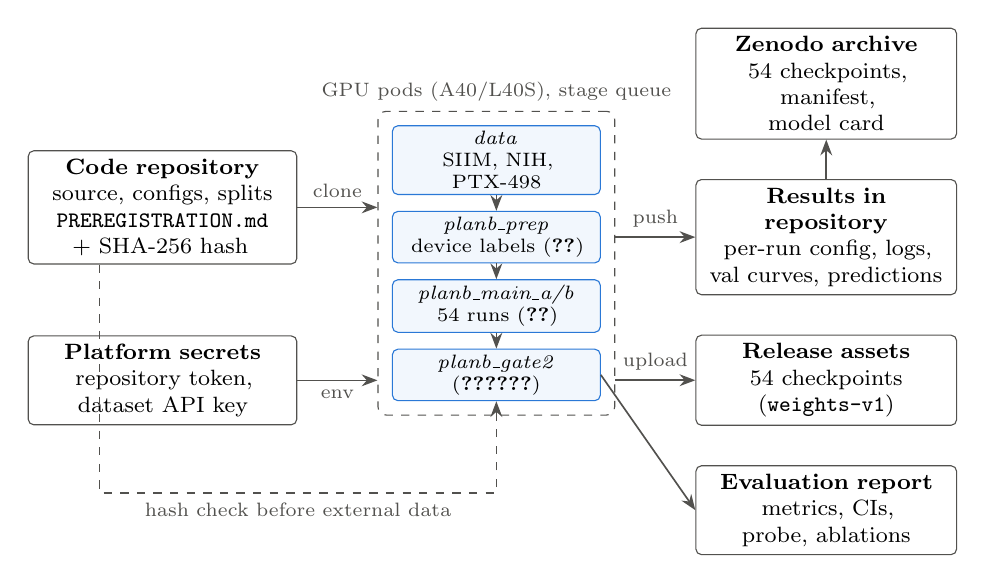
\begin{tikzpicture}[
  node distance=5mm and 7mm,
  box/.style={draw=muted, rounded corners=2pt, align=center, font=\footnotesize, inner sep=3pt, text width=#1, fill=white},
  box/.default=3.3cm,
  st/.style={draw=accent, rounded corners=2pt, align=center, font=\scriptsize, inner sep=2pt, text width=2.5cm, fill=accent!6},
  arr/.style={-{Stealth[length=2mm]}, draw=muted, line width=0.6pt},
  lab/.style={font=\scriptsize, text=muted}]
\node[box=3.2cm] (repo) {\textbf{Code repository}\\ source, configs, splits\\ \texttt{PREREGISTRATION.md}\\ + SHA-256 hash};
\node[box=3.2cm, below=9mm of repo] (secrets) {\textbf{Platform secrets}\\ repository token,\\ dataset API key};
\node[st, right=12mm of repo, yshift=6mm] (s1) {\emph{data}\\ SIIM, NIH, PTX-498};
\node[st, below=2mm of s1] (s2) {\emph{planb\_prep}\\ device labels (\cref{alg:pseudo})};
\node[st, below=2mm of s2] (s3) {\emph{planb\_main\_a/b}\\ 54 runs (\cref{alg:train})};
\node[st, below=2mm of s3] (s4) {\emph{planb\_gate2}\\ (\cref{alg:score,alg:eval,alg:boot})};
\begin{scope}[on background layer]
\node[draw=muted, dashed, rounded corners=3pt, fit=(s1)(s4), inner sep=5pt, label={[lab]above:GPU pods (A40/L40S), stage queue}] (pod) {};
\end{scope}
\node[box=3.1cm, right=12mm of s2] (res) {\textbf{Results in repository}\\ per-run config, logs,\\ val curves, predictions};
\node[box=3.1cm, below=5mm of res] (rel) {\textbf{Release assets}\\ 54 checkpoints\\ (\texttt{weights-v1})};
\node[box=3.1cm, below=5mm of rel] (rep) {\textbf{Evaluation report}\\ metrics, CIs,\\ probe, ablations};
\node[box=3.1cm, above=5mm of res] (zen) {\textbf{Zenodo archive}\\ 54 checkpoints, manifest,\\ model card};
\draw[arr] (repo.east) -- node[lab, above, sloped]{clone} (pod.west |- repo.east);
\draw[arr] (secrets.east) -- node[lab, below, sloped]{env} (pod.west |- secrets.east);
\draw[arr] (s1) -- (s2); \draw[arr] (s2) -- (s3); \draw[arr] (s3) -- (s4);
\draw[arr] (pod.east |- res.west) -- node[lab, above]{push} (res.west);
\draw[arr] (pod.east |- rel.west) -- node[lab, above]{upload} (rel.west);
\draw[arr] (s4.east) -- (rep.west);
\draw[arr] (res) -- (zen);
\draw[arr, dashed] (repo.south) ++(-0.8,0) -- ++(0,-2.9) -| node[lab, pos=0.25, below]{hash check before external data} (s4.south);
\end{tikzpicture}
\caption{System architecture. Every stage runs from the versioned repository on disposable GPU pods; results flow back to the repository, checkpoints to release assets. The evaluation stage verifies the frozen protocol hash before opening external data.}
\label{fig:system}
\end{figure*}

\subsection{Data}
\label{sec:data}
\Cref{tab:data} lists the datasets and their roles, and \cref{fig:examples} shows examples.

\textbf{SIIM-ACR} \cite{siim2019kaggle} (10{,}675 radiographs with labels, 2{,}379 with pneumothorax and segmentation masks) was the development set. It was split 70/10/20 into train (7{,}474), validation (1{,}067) and internal test (2{,}134) with a fixed seed (2026). The 70/10/20 ratio was fixed in the protocol. It is a conventional partition that keeps most images for training while leaving a validation set large enough to place the 95\%-specificity threshold on more than 800 negatives and an internal test set of more than 2{,}000 images; it was not tuned. SIIM-ACR releases one identifier per image and no patient identifier, so splitting was at image level, with near-duplicates (perceptual hash, Hamming distance $\le 4$) grouped into the same split. The consequences of image-level splitting are quantified in \cref{sec:dependencies}.

\textbf{NIH device cohort} \cite{zamora2026cohort} is a curated, patient-wise pneumothorax versus no-finding cohort derived from NIH ChestX-ray14 \cite{wang2017chestxray8}. It contains 4{,}388 radiographs (2{,}194 pneumothorax) with human visible-device annotations and a fixed patient-wise split. Its released \emph{test} split (878 images) was the primary external set. Because SIIM-ACR images were also drawn from ChestX-ray14, we removed from this test split every image with a near-duplicate in SIIM-ACR (357 images). This left 521 images: 125 with pneumothorax (89 with a visible device, 36 without) and 396 without (157 with a device, 238 without, 1 unlabelled). The cohort's train and validation splits were used only for the device classifier and a pilot, never for training pneumothorax models.

\textbf{PTX-498} \cite{wang2021ptx498,wang2021deepsdm} (version v2-fix) contains 498 pneumothorax radiographs with masks from three hospitals. After removing 16 near-duplicates of development images, 482 remained. It contains only positives and has no device annotations. It therefore supports sensitivity, Dice and size endpoints only and provides no specificity, AUROC or device-stratified estimate; the NIH test set is the only external classification evaluation in this study.

\textbf{Image preprocessing.} SIIM-ACR images are distributed as DICOM secondary-capture objects with 8-bit, lossy-compressed pixel data. The pixel array was read with pydicom, inverted when the photometric interpretation was MONOCHROME1, rescaled linearly between its 0.5th and 99.5th intensity percentiles, clipped and stored as 8-bit grayscale. NIH ChestX-ray14 and PTX-498 images are distributed as 8-bit grayscale PNG files and were read without further intensity transformation. No windowing or histogram equalisation was applied. Every image was resized once to $512\times512$ pixels with area interpolation (OpenCV \texttt{INTER\_AREA}); reference masks were resized with area interpolation of the binary mask followed by thresholding at 0.5. At training and inference the grayscale image was replicated to three channels, scaled to $[0,1]$ and normalised with the ImageNet channel means and standard deviations. This normalisation was used for all models, including RAD-DINO, whose inputs were further resized to $518\times518$ by bilinear interpolation inside the model. Geometric augmentation (\cref{sec:training}) used bilinear interpolation with zero padding for images and nearest-neighbour interpolation for masks.

\begin{table*}[!t]
\centering\small
\caption{Datasets and roles in the Plan B analysis.}
\label{tab:data}
\begin{tabularx}{\linewidth}{@{}l p{3.6cm} X r@{}}
\toprule
Dataset & Role & Labels used & Images \\
\midrule
SIIM-ACR & Development (train/val/internal test) & Pneumothorax masks; device \emph{pseudo}-labels (\cref{alg:pseudo}) & 10{,}675 \\
NIH device cohort, released test & Primary external & Pneumothorax vs no finding; human visible-device labels & 521 \\
NIH device cohort, released train/val & Device classifier only & Visible device (uncertain excluded) & 2{,}626 / 875 \\
PTX-498 (v2-fix) & Secondary external (positives only) & Pneumothorax masks, 3 sites & 482 \\
\bottomrule
\end{tabularx}
\end{table*}

\subsection{Dependencies between datasets}
\label{sec:dependencies}
The evaluation is external with respect to the pneumothorax model: no NIH image was used to train, select or threshold any pneumothorax model. It is not independent at the level of the whole pipeline, and \cref{tab:depend} lists the dependencies. First, the device classifier that produced the SIIM-ACR pseudo-labels was trained and thresholded on the NIH cohort's released train and validation splits. These splits are patient-disjoint from the NIH test split by the cohort's design, which we confirmed from the ChestX-ray14 patient identifiers (no NIH test patient appears in them); the three near-duplicate image pairs between these splits and the test split reported in \cref{sec:res-sanity} therefore involve different patients with near-identical images. Second, SIIM-ACR and the NIH cohort are both derived from ChestX-ray14 \cite{wang2017chestxray8}. Image-level near-duplicates of SIIM-ACR images were removed from the NIH test split, but other radiographs of the same patients can remain.

Because SIIM-ACR carries no patient identifier, patient overlap cannot be measured directly. It can be measured on the subset of SIIM-ACR images that match an NEATX-annotated ChestX-ray14 image \cite{jimenez2023shortcuts} by perceptual hash (Hamming distance $\le 4$), since ChestX-ray14 file names encode the patient. Of the 10{,}675 SIIM-ACR images, 2{,}597 matched at least one such image and 2{,}564 matched images of a single patient (860 patients). Within this subset, 323 patients had images in more than one SIIM-ACR split, and 415 of 498 mapped internal-test images (83\%) belonged to a patient who also had images in the training or validation split. Internal-test and validation estimates on SIIM-ACR are therefore optimistic, and the validation set used for checkpoint selection and thresholding is not patient-independent of the training set. For the NIH test split, 46 of its 486 patients (75 of 521 images) had a mapped SIIM-ACR training or validation image. Because the mapping covers only NEATX-annotated images, these counts are lower bounds. The original leakage audit, which reported no patient overlap between SIIM-ACR splits, was uninformative for this reason: it compared per-image identifiers. A sensitivity analysis that excludes the 75 NIH test images is reported in \cref{sec:res-overlap}.

\begin{table*}[!t]
\centering\small
\caption{Dependencies between the data used to build and to evaluate the pipeline. ``Overlap'' counts are from the perceptual-hash mapping of SIIM-ACR images onto NEATX-annotated ChestX-ray14 images and are lower bounds.}
\label{tab:depend}
\begin{tabularx}{\linewidth}{@{}p{3.2cm} p{3.6cm} X@{}}
\toprule
Component & Data used & Relation to the NIH test split (521 images, 486 patients) \\
\midrule
Pneumothorax models (54 runs) & SIIM-ACR train/validation & No NIH image used. Same source archive (ChestX-ray14); image near-duplicates removed; 46 NIH test patients (75 images) have mapped SIIM-ACR development images \\
Checkpoint selection, threshold & SIIM-ACR validation & As above; 83\% of mapped SIIM-ACR internal-test images share a patient with training or validation \\
Device classifier (pseudo-labels) & NIH cohort pilot train/validation & Patient-disjoint from the NIH test split (verified); same cohort, same device annotation protocol \\
Device labels at evaluation & NIH cohort human annotations & Used only for stratification, never for training \\
Chest-drain labels (NEATX) & ChestX-ray14 subset & Used only for post hoc validation analyses \\
\bottomrule
\end{tabularx}
\end{table*}

\subsection{Device pseudo-labels}
\label{sec:pseudo}
\Cref{alg:pseudo} specifies the labelling step. An EfficientNet-B0 \cite{tan2019efficientnet} (timm implementation, ImageNet weights) was trained for eight epochs at 384~px on the NIH cohort's training split (2{,}626 images with a certain device label), with binary cross-entropy, AdamW (learning rate $3\times10^{-4}$, weight decay $10^{-4}$), a one-cycle learning-rate schedule, batch size 32, mixed precision, the augmentation of \cref{sec:training} and random seed 0. The epoch with the best validation AUROC was kept, and the cut-off maximising balanced accuracy was chosen on the validation split (875 images). Validation AUROC was 0.982, with sensitivity 0.956 and specificity 0.957 at the cut-off (0.398). Applied to SIIM-ACR, it labelled 62.3\% of images as device-bearing: 86.9\% of pneumothorax-positive and 55.3\% of negative images. The label targets any visible device (chest drain, central line, pacemaker, electrocardiogram lead or other hardware), not the chest drain specifically. Throughout the paper, ``device-absent'' therefore means ``no device predicted'' in SIIM-ACR and ``no visible device'' according to the human annotations in the NIH test set. Device absence is an imaging characteristic; it does not establish that a patient has not been treated, and treatment status was not available for any dataset.

No manual audit of the pseudo-labels was performed. Their validity on SIIM-ACR was assessed post hoc against an independent reference: the NEATX chest-drain annotations of ChestX-ray14 pneumothorax images \cite{jimenez2023shortcuts}, transferred by perceptual-hash matching (\cref{sec:dependencies}) to 2{,}578 SIIM-ACR images with an unambiguous drain label. NEATX labels are aggregated non-expert annotations of drains only, so this comparison estimates how often drains are captured by the device label and how much of the device label consists of other hardware; it cannot estimate the accuracy of the label for non-drain devices.

\begin{algorithm}[!t]
\caption{Device pseudo-labelling (stage \emph{planb\_prep})}
\label{alg:pseudo}
\begin{algorithmic}[1]
\Require NIH cohort train split $\mathcal{T}$ and validation split $\mathcal{V}$ with device labels $d\in\{0,1\}$ (uncertain labels removed); SIIM-ACR images $\mathcal{S}$
\Ensure Device pseudo-label $\hat d(x)$ for every $x\in\mathcal{S}$
\State Initialise EfficientNet-B0 $f_\phi$ from ImageNet weights; resize inputs to $384\times384$
\For{$e = 1,\dots,8$}
  \State Train $f_\phi$ one epoch on $\mathcal{T}$ with $\BCE(f_\phi(x),d)$
  \State $a_e \gets \AUC\big(\{d\},\{f_\phi(x)\}\big)$ on $\mathcal{V}$; keep $\phi^\star \gets \phi$ if $a_e$ is the best so far \label{line:pseudo-select}
\EndFor
\State $t^\star \gets \arg\max_t \tfrac12\big(\mathrm{sens}_{\mathcal{V}}(t)+\mathrm{spec}_{\mathcal{V}}(t)\big)$ using $f_{\phi^\star}$ \label{line:pseudo-thr}
\For{each $x\in\mathcal{S}$ (all splits)}
  \State $\hat d(x) \gets \mathbf{1}\big[\sigma(f_{\phi^\star}(x)) \ge t^\star\big]$
\EndFor
\State \Return $\hat d$ \Comment{NIH \emph{test} split is never touched}
\end{algorithmic}
\end{algorithm}

\subsection{Proposed model}
\label{sec:model}
\Cref{fig:arch} shows the network. An input radiograph $x\in\mathbb{R}^{3\times H\times W}$ ($H=W=512$) passes through an EfficientNet-B4 encoder $E$ that returns five feature maps $F_1,\dots,F_5$, and a U-Net decoder $D$ \cite{ronneberger2015unet} with skip connections that returns pixel logits
\begin{equation}
Z = D(F_1,\dots,F_5)\in\mathbb{R}^{H\times W}.
\label{eq:seg}
\end{equation}
Let $h=\GAP(F_5)\in\mathbb{R}^{c}$ be the globally average-pooled deepest feature map ($c=448$ for EfficientNet-B4).

\paragraph{C4: mask pooling}
The image-level logit is computed from the segmentation map alone:
\begin{equation}
\begin{aligned}
s(x) &= a\cdot\frac{1}{k}\sum_{(i,j)\in\topk(Z)} Z_{ij} + b,\\
k &=\max\big(1,\lfloor\rho HW\rfloor\big),\quad \rho=0.005,
\end{aligned}
\label{eq:maskpool}
\end{equation}
where $\topk(Z)$ indexes the $k$ largest pixel logits ($k=1{,}310$ at 512~px) and $a,b$ are learned scalars initialised to $1$ and $0$. Without C4, a global head is used instead: $s(x)=w^\top \mathrm{Dropout}(h)+b$.

\paragraph{C2: device adversary}
A gradient-reversal layer $R_\lambda$ \cite{ganin2015dann} is the identity in the forward pass and multiplies gradients by $-\lambda$ in the backward pass:
\begin{equation}
R_\lambda(h)=h,\qquad \frac{\partial R_\lambda(h)}{\partial h}=-\lambda I.
\label{eq:grl}
\end{equation}
A two-layer perceptron $g_\psi$ (256 hidden units, ReLU, dropout 0.2) predicts the device label from $R_\lambda(h)$, giving $\hat d = g_\psi(R_\lambda(h))$. The adversary minimises its loss; because of \cref{eq:grl}, the encoder receives the negated gradient and is pushed to make $h$ uninformative about the device. We used $\lambda=0.1$.

\paragraph{Losses}
For a mini-batch $\mathcal{B}$ with pneumothorax labels $y$, masks $M$ (available for positives) and device pseudo-labels $\hat d$,
\begin{align}
\mathcal{L}_{\text{cls}} &= \tfrac{1}{|\mathcal{B}|}\textstyle\sum_{n}\BCE\big(s(x_n),y_n\big), \label{eq:lcls}\\
\mathcal{L}_{\text{seg}} &= \BCE_{\text{pix}}(Z,M) + \Big(1-\frac{2\sum Z^\sigma M + \epsilon}{\sum Z^\sigma + \sum M + \epsilon}\Big)_{y=1}, \label{eq:lseg}\\
\mathcal{L}_{\text{adv}} &= \tfrac{1}{|\mathcal{B}|}\textstyle\sum_n\BCE\big(g_\psi(R_\lambda(h_n)),\hat d_n\big), \label{eq:ladv}\\
\mathcal{L} &= \mathcal{L}_{\text{cls}} + w_{\text{seg}}\,\mathcal{L}_{\text{seg}} + w_{\text{adv}}\,\mathcal{L}_{\text{adv}},\qquad w_{\text{seg}}=w_{\text{adv}}=1, \label{eq:ltotal}
\end{align}
where $Z^\sigma$ is the sigmoid of $Z$, the pixel BCE is averaged over images that have a mask (empty masks for negatives), and the soft-Dice term is computed over positives only. \Cref{alg:train} gives the full training procedure and \cref{alg:score} the scoring rule.

\begin{figure*}[!t]
\centering
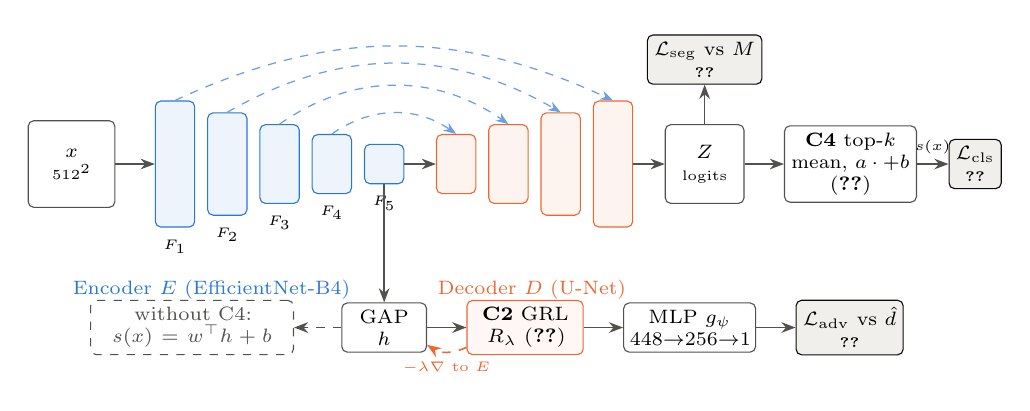
\begin{tikzpicture}[
  node distance=4mm and 5mm,
  blk/.style={draw=muted, rounded corners=2pt, align=center, font=\scriptsize, inner sep=2.5pt, fill=white},
  enc/.style={blk, fill=accent!8, draw=accent, minimum height=#1, minimum width=5mm},
  dec/.style={blk, fill=warm!8, draw=warm, minimum height=#1, minimum width=5mm},
  loss/.style={blk, draw=ink, fill=band, font=\scriptsize},
  arr/.style={-{Stealth[length=1.8mm]}, draw=muted, line width=0.55pt},
  skip/.style={-{Stealth[length=1.6mm]}, draw=accent!70, line width=0.45pt, dashed}]
% input
\node[blk, minimum width=11mm, minimum height=11mm] (x) {$x$\\ \tiny 512$^2$};
% encoder stages
\node[enc=16mm, right=5mm of x] (e1) {};
\node[enc=13mm, right=1.5mm of e1] (e2) {};
\node[enc=10mm, right=1.5mm of e2] (e3) {};
\node[enc=7.5mm, right=1.5mm of e3] (e4) {};
\node[enc=5mm, right=1.5mm of e4] (e5) {};
\node[font=\scriptsize, text=accent] (elab) at ($(e2)+(-0.2,-1.6)$) {Encoder $E$ (EfficientNet-B4)};
\foreach \i in {1,...,5} {\node[font=\tiny, below=0.3mm of e\i] {$F_\i$};}
% decoder
\node[dec=7.5mm, right=4mm of e5] (d4) {};
\node[dec=10mm, right=1.5mm of d4] (d3) {};
\node[dec=13mm, right=1.5mm of d3] (d2) {};
\node[dec=16mm, right=1.5mm of d2] (d1) {};
\node[font=\scriptsize, text=warm] at ($(d3)+(0.3,-1.6)$) {Decoder $D$ (U-Net)};
\draw[arr] (x) -- (e1);
\draw[arr] (e5) -- (d4);
\draw[skip] (e4.north) to[bend left=35] (d4.north);
\draw[skip] (e3.north) to[bend left=35] (d3.north);
\draw[skip] (e2.north) to[bend left=30] (d2.north);
\draw[skip] (e1.north) to[bend left=25] (d1.north);
% seg map
\node[blk, right=4mm of d1, minimum width=10mm, minimum height=10mm] (Z) {$Z$\\ \tiny logits};
\draw[arr] (d1) -- (Z);
% C4
\node[blk, right=5mm of Z, text width=15mm] (tk) {\textbf{C4} top-$k$\\ mean, $a\cdot{+}b$\\ (\cref{eq:maskpool})};
\draw[arr] (Z) -- (tk);
\node[loss, right=4mm of tk] (lcls) {$\mathcal{L}_{\text{cls}}$\\ \tiny \cref{eq:lcls}};
\draw[arr] (tk) -- node[font=\tiny, above]{$s(x)$} (lcls);
\node[loss, above=5mm of Z] (lseg) {$\mathcal{L}_{\text{seg}}$ vs $M$\\ \tiny \cref{eq:lseg}};
\draw[arr] (Z) -- (lseg);
% C2 branch
\node[blk, below=15mm of e5, text width=9mm] (gap) {GAP\\ $h$};
\draw[arr] (e5) -- (gap);
\node[blk, right=5mm of gap, text width=13mm, draw=warm, fill=warm!5] (grl) {\textbf{C2} GRL\\ $R_\lambda$ (\cref{eq:grl})};
\node[blk, right=5mm of grl, text width=15mm] (mlp) {MLP $g_\psi$\\ 448$\to$256$\to$1};
\node[loss, right=5mm of mlp] (ladv) {$\mathcal{L}_{\text{adv}}$ vs $\hat d$\\ \tiny \cref{eq:ladv}};
\draw[arr] (gap) -- (grl); \draw[arr] (grl) -- (mlp); \draw[arr] (mlp) -- (ladv);
\draw[-{Stealth[length=1.8mm]}, draw=warm, line width=0.6pt, dashed] ($(grl.south west)+(0,0.1)$) to[bend left=30] node[font=\tiny, text=warm, below]{$-\lambda\nabla$ to $E$} ($(gap.south east)+(0,0.1)$);
% global head alternative
\node[blk, left=6mm of gap, text width=24mm, draw=muted, dashed, text=muted] (glob) {without C4: $s(x)=w^\top h+b$};
\draw[arr, dashed] (gap.west) -- (glob.east);
\end{tikzpicture}
\caption{Proposed network (C2+C4). The image score is computed from the segmentation logits by top-$k$ mask pooling (C4). A device adversary with gradient reversal (C2) acts on the pooled deepest encoder features $h$. Ablations remove C2, replace C4 by the global head (dashed), or both. Dashed blue arrows are U-Net skip connections.}
\label{fig:arch}
\end{figure*}

\begin{algorithm}[!t]
\caption{Training one configuration with one seed (stages \emph{planb\_main\_a/b})}
\label{alg:train}
\begin{algorithmic}[1]
\Require SIIM-ACR train $\mathcal{D}_{tr}$, validation $\mathcal{D}_{va}$; device pseudo-labels $\hat d$ (\cref{alg:pseudo}); seed $r$; switches C2, C4, DRO
\Ensure Checkpoint $\theta^\star$ and threshold $\tau$
\State Set all random seeds to $r$; initialise $E$ from ImageNet; $\theta\gets(E,D,a,b,g_\psi)$
\State Sampler with replacement, weights such that positives form 50\% of draws
\State AdamW (lr $3\!\times\!10^{-4}$, weight decay $10^{-4}$), 1-epoch linear warm-up then cosine decay; AMP
\State $u^\star\gets-\infty$; \textbf{if} DRO: $q\gets\mathbf{1}/4$ over groups $(y,\hat d)$
\For{$e=1,\dots,20$}
  \For{each mini-batch $\mathcal{B}$ of 16 from the sampler}
    \State Augment: flip, rotation $\pm10^\circ$, scale $0.9$--$1.1$, shift $\pm5\%$, brightness/contrast
    \State Forward: $Z$ by \cref{eq:seg}; $s$ by \cref{eq:maskpool} if C4, else global head
    \State $\mathcal{L}\gets\mathcal{L}_{\text{cls}}+\mathcal{L}_{\text{seg}}$ \Comment{\cref{eq:lcls,eq:lseg}}
    \If{C2} \State $\mathcal{L}\gets\mathcal{L}+\mathcal{L}_{\text{adv}}$ \Comment{\cref{eq:ladv}; reversal by \cref{eq:grl}} \label{line:adv}
    \EndIf
    \If{DRO} \State replace $\mathcal{L}_{\text{cls}}$ by $\sum_g q_g\ell_g$, then $q_g\gets q_g e^{\eta\ell_g}$, renormalise ($\eta=0.01$) \label{line:dro}
    \EndIf
    \State Backward; clip gradient norm at 5; optimiser and scheduler step
  \EndFor
  \State On $\mathcal{D}_{va}$: $\tau_e\gets$ threshold at 95\% specificity (\cref{eq:tau}); $u_e\gets$ device-absent sensitivity at $\tau_e$
  \If{$u_e>u^\star$} \State $u^\star\gets u_e$; $\theta^\star\gets\theta$; $\tau\gets\tau_e$ \label{line:select}
  \EndIf
\EndFor
\State \Return $\theta^\star,\tau$
\end{algorithmic}
\end{algorithm}

\subsection{Ablations and baselines}
\label{sec:baselines}
All pneumothorax models except RAD-DINO use a segmentation network from the Segmentation Models PyTorch library \cite{iakubovskii2019smp} with ImageNet weights and a 512$\times$512 input. \Cref{tab:models} summarises the configurations.

\begin{itemize}
  \item \textbf{Ablations:} C4 only (no adversary); C2 only (global head instead of mask pooling); base (neither). \textbf{Sensitivity runs:} $\lambda=0.01$ and $\lambda=1.0$ with C2 and the global head.
  \item \textbf{Baselines:} U-Net with a ResNet34 encoder \cite{he2016resnet}, a common choice among SIIM-ACR challenge solutions (mask pooling); SegFormer-B2 \cite{xie2021segformer} (mask pooling); Group DRO \cite{sagawa2020groupdro} over four groups (pneumothorax $\times$ device, step size 0.01, \cref{line:dro} of \cref{alg:train}) on the EfficientNet-B4 U-Net; an auxiliary device classifier without gradient reversal (linear head on $h$, loss weight 0.5), after Bandaru et al.~\cite{bandaru2026untreated}; and RAD-DINO \cite{perezgarcia2025raddino} with a linear head on the pooled output at 518~px, either frozen (linear probe; lr $10^{-3}$, batch 32) or fully fine-tuned (lr $2\times10^{-5}$).
\end{itemize}

The protocol listed nnU-Net 2D \cite{isensee2021nnunet} and zero-shot multimodal models as baselines. The Plan B deviations, recorded before freezing, deferred both to secondary comparisons after the main evaluation and excluded them from the ``best baseline'' comparisons; neither was run. nnU-Net is a self-configuring segmentation framework that outputs masks without an image-level score, so its use for the classification endpoints would have required the same top-$k$ pooling rule and would have added a further mask-pooling segmentation baseline alongside U-Net ResNet34 and SegFormer-B2. Its omission, and that of vision--language models, restricts the cross-architecture comparison to supervised convolutional and transformer segmentation networks and a self-supervised foundation-model encoder trained with one recipe; CLIP-based chest radiograph models have been reported separately to perform worse on pneumothorax without drains \cite{sourget2025clip}. Tube-mask components (inpainting and auxiliary tube segmentation) require tube masks and were dropped.

\begin{table*}[!t]
\centering\small
\caption{Model configurations. All were trained on the same SIIM-ACR splits with the same augmentation and schedule (\cref{alg:train}). ``Mask pool'' = \cref{eq:maskpool}; ``Global'' = linear head on $h$.}
\label{tab:models}
\begin{tabular}{@{}l l l l c@{}}
\toprule
Model & Backbone & Image score & Device handling & Seeds \\
\midrule
\textbf{Proposed (C2+C4)} & U-Net / EfficientNet-B4 & Mask pool & Gradient reversal, $\lambda$=0.1 & 5 \\
Ablation: C4 only & U-Net / EfficientNet-B4 & Mask pool & --- & 5 \\
Ablation: C2 only & U-Net / EfficientNet-B4 & Global & Gradient reversal, $\lambda$=0.1 & 5 \\
Ablation: base & U-Net / EfficientNet-B4 & Global & --- & 5 \\
Sensitivity $\lambda$=0.01 / 1.0 & U-Net / EfficientNet-B4 & Global & Gradient reversal & 3 / 3 \\
U-Net ResNet34 & U-Net / ResNet34 & Mask pool & --- & 5 \\
SegFormer-B2 & SegFormer / MiT-B2 & Mask pool & --- & 3 \\
Group DRO & U-Net / EfficientNet-B4 & Mask pool & Worst-group reweighting & 5 \\
Aux.\ device classifier & U-Net / EfficientNet-B4 & Global & Auxiliary head (no reversal) & 5 \\
RAD-DINO linear probe & ViT-B (RAD-DINO), frozen & Global & --- & 5 \\
RAD-DINO fine-tuned & ViT-B (RAD-DINO) & Global & --- & 5 \\
\bottomrule
\end{tabular}
\end{table*}

\subsection{Training, operating point and scoring}
\label{sec:training}
Training followed \cref{alg:train}: 20 epochs, AdamW (learning rate $3\times10^{-4}$, weight decay $10^{-4}$, batch 16), one epoch of linear warm-up followed by cosine decay, gradient clipping at 5, mixed precision and positive oversampling to 50\% of draws. Augmentation was horizontal flipping, rotation ($\pm10^\circ$), scaling (0.9--1.1), translation ($\pm5\%$) and random brightness/contrast. The checkpoint kept was the epoch with the highest device-absent sensitivity at 95\% specificity on SIIM-ACR validation (\cref{line:select}). That set contains only 32 device-absent positives; the stability of this selection is analysed in \cref{sec:res-conv}. Each model's threshold was set at 95\% specificity on the same validation set,
\begin{equation}
\tau = \mathrm{next}\big(v_{(\lceil 0.95\,n_0\rceil)}\big),
\label{eq:tau}
\end{equation}
where $v_{(1)}\le\dots\le v_{(n_0)}$ are the sorted validation scores of the $n_0$ negatives and $\mathrm{next}(\cdot)$ is the next representable number above, and applied unchanged to all other sets (\cref{alg:score}). Runs took about 20--50 minutes each on a single NVIDIA A40 or L40S GPU. The software environment was Python~3.11 and PyTorch~2.4.1 with CUDA~12.4, with segmentation-models-pytorch, timm, Hugging Face transformers (version below 4.50, for RAD-DINO), scikit-learn, OpenCV and pydicom installed from the version constraints in the repository's \texttt{requirements.txt}; the resolved versions of these packages were not recorded separately.

\textbf{Hyper-parameters.} All optimisation settings, the input size, the top-$k$ fraction $\rho$, the loss weights and the adversary architecture were fixed in the protocol before training, from library defaults and common practice for SIIM-ACR segmentation models; none was tuned on SIIM-ACR test data or on external data. The only hyper-parameter varied was the gradient-reversal strength $\lambda$, as pre-registered sensitivity runs ($\lambda=0.01$, $0.1$, $1$; \cref{sec:res-ablation}). The checkpoint epoch was the only quantity selected on data (SIIM-ACR validation). Because no setting was optimised for the development data, the configuration carries no dataset-specific tuning that would have to be repeated elsewhere; conversely, the study does not show that other values of $\rho$, the loss weights or the adversary capacity would change the result, and these remain untested.

\begin{algorithm}[!t]
\caption{Scoring an image with a trained configuration}
\label{alg:score}
\begin{algorithmic}[1]
\Require Image $x$; checkpoints $\{\theta^\star_r\}_{r=1}^{R}$ and thresholds $\{\tau_r\}$ from \cref{alg:train}
\Ensure Seed-averaged probability $\bar p(x)$ and decision $\hat y(x)$
\For{$r=1,\dots,R$}
  \State Resize $x$ to $512^2$ (RAD-DINO: $518^2$); forward pass with $\theta^\star_r$ in evaluation mode
  \If{mask pooling} \State $s_r\gets a\cdot\mathrm{mean}\big(\topk(Z)\big)+b$ \Comment{\cref{eq:maskpool}}
  \Else \State $s_r\gets w^\top h+b$
  \EndIf
  \State $p_r\gets\sigma(s_r)$ \Comment{the adversary $g_\psi$ is not used at inference}
\EndFor
\State $\bar p(x)\gets\frac1R\sum_r p_r$ \Comment{primary analyses use seed-averaged scores}
\State $\bar\tau\gets$ \cref{eq:tau} applied to seed-averaged SIIM-ACR validation scores\label{line:tau-avg}
\State $\hat y(x)\gets\mathbf{1}[\bar p(x)\ge\bar\tau]$ (primary summaries); per-seed $\mathbf{1}[p_r\ge\tau_r]$ for seed-level analyses
\State \Return $\bar p(x),\hat y(x)$
\end{algorithmic}
\end{algorithm}

\subsection{Endpoints}
\label{sec:endpoints}
The two primary endpoints, both on the NIH test set, were device-absent sensitivity at the threshold transferred from SIIM-ACR validation and the device--device-absent AUROC gap. Secondary endpoints were device-absent AUROC (paired DeLong test with Holm correction across baselines \cite{delong1988,holm1979}), sensitivity for small pneumothorax, Dice, agreement of the predicted size class (weighted $\kappa$), calibration after temperature scaling (15-bin ECE \cite{guo2017calibration}) and seed-to-seed stability. Each was compared with the strongest re-trained baseline for that dataset and metric, chosen from U-Net ResNet34, the C4-only EfficientNet-B4 U-Net, SegFormer-B2, Group DRO, the auxiliary device classifier and both RAD-DINO variants; segmentation endpoints used only the segmentation baselines. \Cref{alg:eval} gives the evaluation procedure. With $P_{\text{dev}}$, $P_{\text{abs}}$ and $N$ the device-present positives, device-absent positives and all negatives, the stratified quantities are
\begin{align}
\Delta_{\text{gap}} &= \AUC(P_{\text{dev}},N)-\AUC(P_{\text{abs}},N), \label{eq:gap}\\
\AUC_{\text{dev}\mid y=0} &= \Pr\big[\bar p(x^{+})>\bar p(x^{-})\big], \label{eq:devscore}\\
&\qquad x^{+}\in N_{\text{dev}},\ x^{-}\in N_{\text{none}}, \nonumber
\end{align}
where $\AUC(A,B)$ is the probability that a random member of $A$ scores above a random member of $B$ (ties count one half). \Cref{eq:gap} is a primary endpoint. \Cref{eq:devscore}, the \emph{device-in-score} AUROC, is exploratory: a value above 0.5 means that, among images without pneumothorax, device-bearing images receive higher pneumothorax scores than device-free images.

\paragraph{Device probe, leakage audit and ablations}
\emph{Device probe:} a logistic regression ($\ell_2$ penalty, $C=0.1$) predicting the human device label from each model's pooled encoder features $h$ on the NIH test set, as a measure of residual device information. The probe was fitted and evaluated by stratified 5-fold cross-validation, and the reported AUROC is computed only from held-out-fold predictions; it is averaged over seeds. Folds were assigned by image; because the 521 NIH test images come from 486 patients, at most 35 images can share a patient with an image in another fold. Post hoc, the same probe was applied, with pseudo-labelled device status and with NEATX chest-drain labels as targets, on the SIIM-ACR internal test set, which is drawn from the development distribution. \emph{Leakage audit:} patient overlap across development splits and perceptual-hash near-duplicates between any training-like split and any test split. \emph{Ablations:} each component was removed in turn, and device-absent sensitivity on the NIH test set was compared with the full model using paired seeds and the seed-averaged difference with a bootstrap CI.

\begin{algorithm}[!t]
\caption{Single external evaluation (stage \emph{planb\_gate2})}
\label{alg:eval}
\begin{algorithmic}[1]
\Require Frozen protocol file $\Pi$ and stored hash $H$; all trained runs; external sets NIH test, PTX-498
\Ensure Per-image predictions and the evaluation report
\If{$\mathrm{SHA256}(\Pi)\neq H$} \State \textbf{abort} \Comment{no external data opened} \label{line:hash}
\EndIf
\State Run leakage audit (patients, perceptual-hash near-duplicates across all splits)
\For{each run} \State score every external image once with \cref{alg:score}; store predictions
\EndFor
\State Compute primary and secondary endpoints for every model, with CIs from \cref{alg:boot}
\State Device-absent AUROC: paired DeLong test vs each baseline, Holm correction
\State Calibration: fit temperature on SIIM-ACR validation, then 15-bin ECE on NIH
\State Device probe on pooled features; paired-seed ablation comparisons
\State \Return predictions and report
\end{algorithmic}
\end{algorithm}

\begin{table*}[!t]
\centering\small
\caption{Primary and secondary endpoints for the proposed model and the strongest re-trained comparator for each endpoint. Primary external set = NIH test. Differences are proposed minus comparator with 95\% patient-cluster bootstrap CIs.}
\label{tab:endpoints}
\begin{tabularx}{\linewidth}{@{}>{\raggedright\arraybackslash}p{5.2cm} >{\raggedright\arraybackslash}p{3.4cm} >{\raggedright\arraybackslash}X@{}}
\toprule
Endpoint & Proposed & Strongest comparator; difference \\
\midrule
\multicolumn{3}{@{}l}{\emph{Primary (NIH test)}}\\
Device-absent sensitivity, transferred threshold & 0.222 (8/36) & SegFormer-B2 0.278 (10/36); $-$0.056 \ci{$-$0.143}{0.000} \\
Device--device-absent AUROC gap (\cref{eq:gap}) & 0.258 & Group DRO 0.086 (smallest gap) \\
\midrule
\multicolumn{3}{@{}l}{\emph{Secondary}}\\
Device-absent AUROC (NIH) & 0.695 & RAD-DINO probe 0.816; $-$0.121, DeLong $p_\text{Holm}=0.046$ (clustered 0.023) \\
Small-pneumothorax sensitivity & SIIM 0.636; PTX-498 0.404 & SIIM 0.693 ($n$=225); PTX-498 0.634 ($n$=161) \\
Dice & SIIM 0.460; PTX-498 0.478 & SegFormer-B2: SIIM 0.499; PTX-498 0.731 \\
Size class, weighted $\kappa$ & SIIM 0.375; PTX-498 0.478 & --- \\
ECE after temperature scaling (NIH) & 0.097 ($T$=1.56) & --- \\
Seed SD of device-absent sensitivity & 0.070 & 0/5 seeds above the comparator mean \\
\bottomrule
\end{tabularx}
\end{table*}

\subsection{Statistics}
\label{sec:stats}
Primary analyses use seed-averaged scores. 95\% CIs come from a patient-cluster bootstrap with 2{,}000 resamples (\cref{alg:boot}). Paired differences between models use the same resamples, so that between-model correlation is preserved. Proportions are additionally reported with Wilson score intervals \cite{wilson1927}.

\textbf{Tests.} The pre-specified test is the paired DeLong test of device-absent AUROC between the proposed model and each of the seven re-trained comparators listed in \cref{sec:endpoints}, with Holm adjustment over these seven. Because the 521 NIH test images come from 486 patients, the same comparison was repeated post hoc with the clustered extension of the DeLong test by Obuchowski \cite{obuchowski1997clustered}, which treats the patient as the sampling unit. All other tests are post hoc patient-cluster bootstrap tests. For a paired difference $\delta$ with bootstrap replicates $\delta^{*}_1,\dots,\delta^{*}_B$, the two-sided p-value for the null hypothesis $\delta=0$ is
\begin{equation}
p = \max\!\Big(\tfrac{1}{B},\; 2\min\big\{\tfrac{1}{B}\textstyle\sum_b \mathbf{1}[\delta^{*}_b\le 0],\; \tfrac{1}{B}\textstyle\sum_b \mathbf{1}[\delta^{*}_b\ge 0]\big\}\Big),
\label{eq:pboot}
\end{equation}
which is the smallest level at which the percentile CI excludes zero. Holm adjustment was applied separately for each contrast (device-absent AUROC, gap, device-absent sensitivity and device-in-score AUROC) over the eleven comparisons of the proposed model with every other configuration.

\textbf{Variation between training runs.} The patient-cluster bootstrap treats the trained models as fixed. To include variation between seeds, a two-stage bootstrap \cite{ren2010hierboot} was applied post hoc: in each of 2{,}000 replicates, patients were resampled with replacement (shared by all models) and, independently for each configuration, its 3--5 seeds were resampled with replacement; the seed-averaged scores and the SIIM-ACR validation threshold (\cref{eq:tau}) were recomputed from the resampled seeds. Seed-level endpoints, in which each seed is scored with its own threshold, are summarised by their mean, standard deviation and range. Pneumothorax size follows the British Thoracic Society rim criterion ($\ge$20~mm) where pixel spacing is known, and area-fraction tertiles otherwise \cite{macduff2010bts}.

\paragraph{Exploratory analyses (not pre-registered)} On the NIH test set we computed, for all twelve configurations, AUROC for device-absent and for device-present positives against all negatives; paired differences between the proposed model and each comparator; the device-in-score AUROC (\cref{eq:devscore}); sensitivity at 95\% specificity recalibrated on the NIH set itself (an oracle threshold); an analysis excluding images involved in the leakage finding; per-epoch training and validation curves (\cref{sec:res-conv}); and seed-averaged segmentation maps and Grad-CAM \cite{selvaraju2020gradcam} for examples chosen by fixed rules (\cref{sec:res-qual}). These results are descriptive.

\paragraph{Post hoc analyses} After the exploratory analyses above, and without retraining or re-thresholding any model, the following analyses were performed: (i) severity-stratified device--device-absent AUROC differences on the SIIM-ACR internal test set, using reference-mask area tertiles, and a size-adjusted regression of the image logit on device status among positives; (ii) stratification of the NIH test set by view position and adjustment for view position, sex and age, from the ChestX-ray14 metadata; (iii) the NEATX pseudo-label comparison (\cref{sec:pseudo}) and drain-specific strata on both test sets; (iv) the patient-overlap mapping and an exclusion analysis (\cref{sec:dependencies}); (v) the overlap of the top-$k$ pixels with the reference pneumothorax mask (\cref{sec:res-topk}); (vi) score-distribution analyses of threshold transfer; (vii) the device probe on the development distribution; (viii) paired differences with Holm adjustment for all three primary and secondary contrasts; and (ix) computational cost. Analyses (v), (vii) and (ix) re-ran the released checkpoints once in inference mode; the re-computed logits were compared with the stored ones as a reproducibility check. A second set of post hoc analyses used only stored predictions and logs: (x) seed-level summaries, the two-stage bootstrap and the clustered DeLong test; (xi) all endpoints with CIs after exclusion of the identified patient overlap; (xii) Wilson and patient-cluster intervals for the pseudo-label comparison and a comparison of the mapped subset with the remaining SIIM-ACR images; (xiii) the stability of checkpoint selection from the per-epoch logs; and (xiv) acquisition-related metadata on NIH. All are exploratory and are reported as such.

\Cref{tab:protocol} gives the order of the protocol versions and analyses with immutable identifiers. Commit hashes refer to the public code repository; a commit hash is a cryptographic digest of the repository content, so the protocol text and analysis code at each stage can be retrieved and verified, and the frozen protocol file can additionally be checked against its recorded SHA-256 digest.

\begin{table*}[!t]
\centering\small
\caption{Protocol versions and analysis hierarchy. ``Commit'' is the UTC commit time recorded in the repository; ``Pushed'' is the UTC time at which the repository host (GitHub) received the commit, from its activity record, which repository users cannot edit. Commit hashes are abbreviated to 12 characters. The history after 2 November 2026 was rewritten once, on 16 November, to remove files unrelated to the analysis; all earlier commits, including every protocol commit, are unchanged, and the rewrite appears in the activity record as a forced push.}
\label{tab:protocol}
\begin{tabularx}{\linewidth}{@{}p{3.3cm} l l l X@{}}
\toprule
Stage & Hash & Commit (2026) & Pushed (2026) & Content \\
\midrule
Protocol draft v0.2 & \texttt{b9ac511be2b3} & 23 Sep 11:01:10 & 23 Sep 11:01:10 & Hypotheses, endpoints, pass criteria, baselines and statistics (CANDID-PTX design) \\
Amendment 1 (Plan B) & \texttt{1df4a16c09a3} & 23 Sep 17:44:04 & 23 Sep 17:44:04 & SIIM-ACR development set and device pseudo-labels \\
Deviations recorded & \texttt{0eebef2489c8} & 24 Sep 18:38:43 & 24 Sep 18:38:43 & nnU-Net and zero-shot baselines deferred; tube-mask components dropped \\
Protocol frozen & \texttt{1432ac215d9d} & 24 Sep 23:08:52 & 24 Sep 23:08:55 & SHA-256 of \texttt{PREREGISTRATION.md}: \texttt{0c4f0c756a62\ldots afa5} \\
First external evaluation & \texttt{58daf122c7f3} & 24 Sep 23:24:29 & 24 Sep 23:24:36 & External predictions written once per model (pre-specified primary, secondary and sanity analyses) \\
Acceptance report & \texttt{8e6566e50aba} & 25 Sep 00:18:00 & 25 Sep 00:18:04 & Pre-specified pass/fail evaluation \\
Exploratory analyses & --- & after 25 Sep & --- & Stratified AUROCs, paired differences, device-in-score, oracle threshold, curves, maps \\
Post hoc analyses & \texttt{6f9c09e2f31f} & 2 Nov 02:07:46 & 2 Nov 02:07:48 & Analyses (i)--(ix) above \\
Post hoc analyses & \texttt{681f2c71274f} & 16 Nov 11:37:05 & 16 Nov 11:48:52 & Analyses (x)--(xiv) above \\
\bottomrule
\end{tabularx}
\end{table*}

\begin{algorithm}[!t]
\caption{Patient-cluster bootstrap for CIs and paired differences}
\label{alg:boot}
\begin{algorithmic}[1]
\Require Test images with patient IDs; seed-averaged scores $\bar p^{(m)}$ for every model $m$; statistic $T$ (e.g.\ \cref{eq:gap,eq:devscore}); $B=2000$
\Ensure Point estimates and 95\% CIs for $T^{(m)}$ and for $T^{(\text{prop})}-T^{(m)}$
\State Group image indices by patient: $\mathcal{C}_1,\dots,\mathcal{C}_K$; fix the random generator (seed 0)
\State $\hat T^{(m)}\gets T\big(\bar p^{(m)}\big)$ on all images
\For{$b=1,\dots,B$}
  \State Draw $K$ patients with replacement; $I_b\gets$ concatenation of their image indices
  \For{each model $m$} \State $T^{(m)}_b\gets T\big(\bar p^{(m)}[I_b]\big)$ \Comment{same $I_b$ for all models}
  \EndFor
  \State $\delta^{(m)}_b\gets T^{(\text{prop})}_b-T^{(m)}_b$
\EndFor
\State Drop undefined replicates (e.g.\ a stratum absent from $I_b$)
\State $p^{(m)}\gets$ \cref{eq:pboot} applied to $\{\delta^{(m)}_b\}$; Holm adjustment over the comparators $m$
\State \Return $\hat T^{(m)}$, percentiles 2.5/97.5 of $\{T^{(m)}_b\}$ and of $\{\delta^{(m)}_b\}$, and $p^{(m)}$
\end{algorithmic}
\end{algorithm}

%% ============================================================ RESULTS
\section{Results}
\label{sec:results}

\subsection{Primary and secondary endpoints}
\label{sec:res-endpoints}
All 54 runs completed. The proposed model did not improve on the strongest comparator for any endpoint (\cref{tab:endpoints}). On the NIH test set its device-absent sensitivity at the transferred threshold was 0.222 (8 of 36 device-absent positives detected; Wilson 95\% CI 0.12--0.38), against 0.278 for SegFormer-B2 (10 of 36; 0.16--0.44). This difference corresponds to two cases; its 95\% CI ($-$0.143 to 0.000) reaches zero, and in the paired analysis eight cases were detected by both models and two by SegFormer-B2 alone. The data therefore show that the proposed model failed to demonstrate superiority on this endpoint; they do not establish that it is inferior. They do not establish equivalence either: equivalence would require the CI of the difference to lie within a pre-specified margin, and with a lower limit of $-$0.143 it would fail for any margin narrower than 14 percentage points. With 36 device-absent positives, the individual sensitivities of all configurations have CIs about 0.25 wide and overlap extensively (\cref{tab:nih}). Its AUC gap (\cref{eq:gap}) of 0.258 was three times that of the smallest-gap baseline (Group DRO, 0.086). Its device-absent AUROC (0.695) was the lowest point estimate of the twelve configurations; the difference from the best baseline (RAD-DINO linear probe, 0.816) was significant after Holm adjustment (pre-specified paired DeLong test, $p_\text{Holm}=0.046$; its clustered extension, which accounts for repeated images of the same patient, gives $p_\text{Holm}=0.023$, and the post hoc paired patient-cluster bootstrap $p_\text{Holm}=0.011$). Only 3 of the 429 patients in this analysis contributed more than one image, so the clustering had little effect. These tests treat the trained models as fixed; when variation between training seeds was included, the CI of the difference was $-$0.277 to $-$0.009 and the Holm-adjusted p-value 0.25 (\cref{sec:res-seeds}). Across seeds, the proposed model's device-absent sensitivity ranged from 0.08 to 0.25 (SD 0.070; \cref{fig:seeds}). On the segmentation and size endpoints SegFormer-B2 performed better (PTX-498 Dice 0.731 versus 0.478). Calibration after temperature scaling was moderate (ECE 0.097). \Cref{tab:nih} gives NIH results for all models, \cref{tab:secondary} internal-test and PTX-498 results, and \cref{fig:heatmap} an overview.

\begin{table*}[!t]
\centering\small
\setlength{\tabcolsep}{3.5pt}
\caption{NIH test set (primary external; 521 images, 125 positives of which 36 device-absent). AUROCs use seed-averaged scores with 95\% patient-cluster bootstrap CIs (\cref{alg:boot}). Sensitivity and specificity are computed from seed-averaged scores at each model's threshold transferred from SIIM-ACR validation (\cref{line:tau-avg} of \cref{alg:score}), with Wilson 95\% CIs for sensitivity; they differ from the means of per-seed values in \cref{tab:ablation,tab:seeds}. ``Device-in-score'' = \cref{eq:devscore} among the 395 labelled negatives (0.5 = no device signal; exploratory). Bold: best value in each column (highest AUROC and sensitivity, lowest gap, device-in-score closest to 0.5).}
\label{tab:nih}
\begin{tabular}{@{}l c c c c c c c@{}}
\toprule
Model & AUROC & \multicolumn{2}{c}{AUROC vs all negatives} & Gap & Device-in- & \multicolumn{2}{c}{At transferred thr.} \\
\cmidrule(lr){3-4}\cmidrule(l){7-8}
 & & Device-absent & Device & (\cref{eq:gap}) & score & Sens.\ dev.-abs. & Spec. \\
\midrule
\rowcolor{band}\textbf{Proposed (C2+C4)} & 0.879 & 0.695 \ci{0.58}{0.81} & 0.954 & 0.258 \ci{0.15}{0.37} & 0.710 & 0.222 \ci{0.12}{0.38} & 1.000 \\
C4 only & 0.881 & 0.745 \ci{0.65}{0.84} & 0.936 & 0.191 \ci{0.09}{0.29} & 0.592 & 0.250 \ci{0.14}{0.41} & 1.000 \\
C2 only & 0.873 & 0.760 \ci{0.67}{0.84} & 0.919 & 0.159 \ci{0.06}{0.25} & \textbf{0.491} & \textbf{0.278} \ci{0.16}{0.44} & 1.000 \\
Base (neither) & 0.870 & 0.815 \ci{0.72}{0.89} & 0.892 & \textbf{0.077} \ci{$-$0.02}{0.18} & 0.477 & 0.250 \ci{0.14}{0.41} & 1.000 \\
$\lambda$=0.01 (C2) & 0.887 & 0.774 \ci{0.67}{0.87} & 0.933 & 0.159 \ci{0.05}{0.26} & 0.559 & --- & --- \\
$\lambda$=1.0 (C2) & 0.860 & 0.738 \ci{0.63}{0.84} & 0.910 & 0.172 \ci{0.06}{0.29} & 0.545 & --- & --- \\
\midrule
U-Net ResNet34 & 0.888 & 0.757 \ci{0.65}{0.86} & 0.941 & 0.185 \ci{0.08}{0.29} & 0.639 & 0.139 \ci{0.06}{0.29} & 1.000 \\
SegFormer-B2 & 0.903 & 0.809 \ci{0.72}{0.89} & 0.941 & 0.133 \ci{0.05}{0.22} & 0.565 & \textbf{0.278} \ci{0.16}{0.44} & 0.998 \\
Group DRO & 0.870 & 0.809 \ci{0.71}{0.90} & 0.895 & 0.086 \ci{$-$0.02}{0.19} & 0.416 & 0.222 \ci{0.12}{0.38} & 0.995 \\
Aux.\ device classifier & 0.881 & 0.757 \ci{0.65}{0.87} & 0.931 & 0.173 \ci{0.06}{0.29} & 0.642 & 0.250 \ci{0.14}{0.41} & 1.000 \\
RAD-DINO probe & \textbf{0.916} & \textbf{0.816} \ci{0.73}{0.89} & 0.956 & 0.140 \ci{0.06}{0.23} & 0.609 & 0.111 \ci{0.04}{0.25} & 0.992 \\
RAD-DINO fine-tuned & 0.908 & 0.803 \ci{0.70}{0.89} & 0.951 & 0.148 \ci{0.05}{0.25} & 0.698 & 0.167 \ci{0.08}{0.32} & 0.998 \\
\bottomrule
\end{tabular}
\end{table*}

\begin{table*}[!t]
\centering\small
\setlength{\tabcolsep}{4.5pt}
\caption{SIIM-ACR internal test (2{,}134 images; 476 positives, 62 without a predicted device) and PTX-498 (482 positives). Seed-averaged; thresholds from SIIM-ACR validation. Device-absent status on SIIM-ACR is a pseudo-label. The internal test set shares patients with the training and validation sets (\cref{sec:dependencies}), so its results describe in-distribution performance and are not evidence of generalisation. PTX-498 contains only positives and supports sensitivity and Dice, not specificity or AUROC. RAD-DINO models have no segmentation output. Bold: best value in each column.}
\label{tab:secondary}
\begin{tabular}{@{}l c c c c c c c@{}}
\toprule
 & \multicolumn{5}{c}{SIIM-ACR internal test} & \multicolumn{2}{c}{PTX-498} \\
\cmidrule(lr){2-6}\cmidrule(l){7-8}
Model & AUROC & Sens. & Spec. & Sens.\ dev.-abs. & Dice & Sens. & Dice \\
\midrule
\rowcolor{band}\textbf{Proposed (C2+C4)} & 0.957 & 0.708 & \textbf{0.963} & 0.548 & 0.460 & 0.693 & 0.478 \\
C4 only & 0.957 & 0.721 & 0.960 & 0.548 & 0.453 & 0.734 & 0.496 \\
C2 only & 0.950 & 0.746 & 0.951 & 0.613 & 0.508 & 0.714 & 0.730 \\
Base (neither) & 0.955 & 0.721 & 0.953 & 0.548 & 0.477 & 0.660 & 0.643 \\
\midrule
U-Net ResNet34 & 0.954 & 0.668 & 0.958 & 0.452 & 0.453 & 0.622 & 0.485 \\
SegFormer-B2 & \textbf{0.959} & \textbf{0.761} & 0.956 & \textbf{0.694} & 0.499 & \textbf{0.830} & \textbf{0.731} \\
Group DRO & 0.952 & 0.691 & 0.961 & 0.613 & 0.458 & 0.782 & 0.595 \\
Aux.\ device classifier & 0.956 & 0.731 & 0.957 & 0.581 & \textbf{0.523} & 0.643 & 0.699 \\
RAD-DINO probe & 0.915 & 0.557 & 0.940 & 0.194 & --- & 0.382 & --- \\
RAD-DINO fine-tuned & 0.949 & 0.716 & 0.940 & 0.629 & --- & 0.635 & --- \\
\bottomrule
\end{tabular}
\end{table*}

\begin{figure*}[!t]
\centering
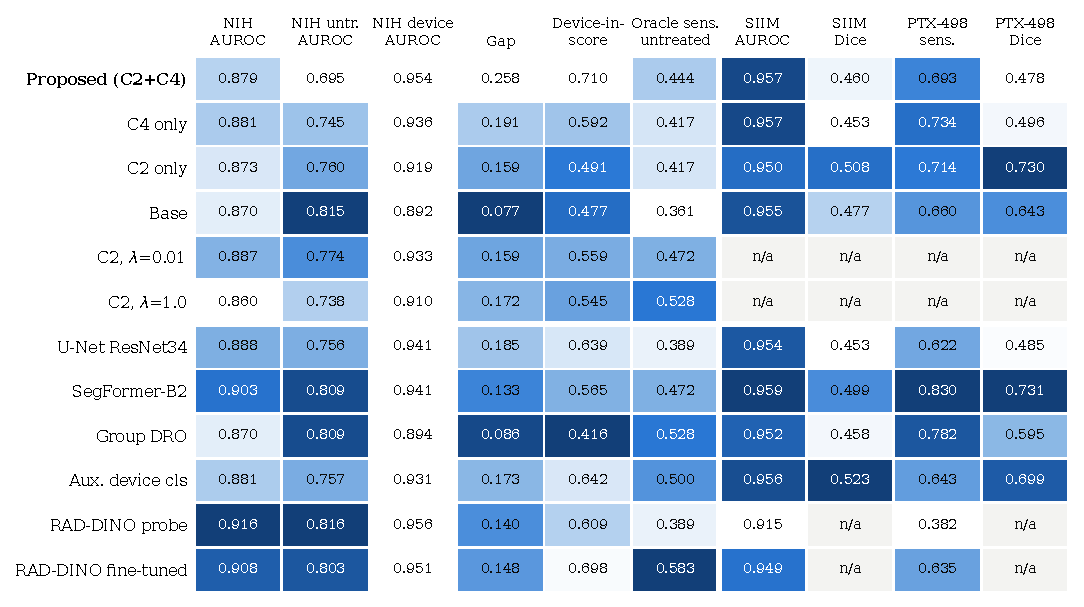
\includegraphics[width=\linewidth]{figures/fig_heatmap.pdf}
\caption{Model $\times$ metric overview. Cells show point estimates; colour encodes the within-column rank (darker = better; for the gap and device-in-score, lower is better). The NIH device-positive AUROC column is left uncoloured because a higher value there can reflect device-associated bias. ``Oracle sens.\ device-absent'' uses a threshold recalibrated on NIH at 95\% specificity. n/a: not computed for the sensitivity runs or no segmentation output.}
\label{fig:heatmap}
\end{figure*}

\subsection{Device probe and leakage audit}
\label{sec:res-sanity}
The proposed model's pooled features still predicted device status on the NIH test set with a held-out-fold probe AUROC of 0.900. This was lower than for the auxiliary device classifier (0.973) and both RAD-DINO models (0.965, 0.960), but higher than for U-Net ResNet34 (0.845) and SegFormer-B2 (0.885). The adversary therefore did not remove device information from the representation.

The pre-specified leakage audit found zero patient overlap between SIIM-ACR splits and four cross-split near-duplicate pairs. The first finding is not informative, because SIIM-ACR assigns a distinct identifier to every image; the post hoc patient-level mapping shows substantial overlap (\cref{sec:dependencies,sec:res-overlap}). Of the four near-duplicate pairs, none involves SIIM-ACR; all involve the NIH cohort's own released splits. Three pair an NIH \emph{pilot-training} image with an NIH \emph{test} image, and one pairs an NIH \emph{pilot-validation} image with PTX-498 image SiteA\_98. None involves SIIM-ACR training or validation data, and the NIH pilot splits were used only to train the device classifier. The three NIH test images are all pneumothorax-negative. Excluding them changed no estimate by more than 0.001 (the proposed model's device-absent AUROC stayed at 0.695 and its gap moved from 0.258 to 0.259).

\subsection{Pseudo-labels against chest-drain annotations (post hoc)}
\label{sec:res-pseudo}
On the 2{,}578 SIIM-ACR images with a transferred NEATX drain label (877 ChestX-ray14 patients), the device pseudo-label was positive for 97.9\% of images with an annotated chest drain (1{,}138 of 1{,}162; Wilson 95\% CI 97.0--98.6\%, patient-cluster bootstrap 97.0--98.7\%), 99.1\% of pneumothorax-positive (98.2--99.5\%) and 94.9\% of pneumothorax-negative images (91.8--96.8\%). Chest drains were therefore almost always inside the attribute that the adversary was trained to remove. The attribute was, however, much broader than chest drains: only 58.9\% of pseudo-labelled device-bearing images had an annotated drain (1{,}138 of 1{,}932; 56.7--61.1\%, cluster bootstrap 54.6--63.0\%), and 56.1\% of images without a drain were labelled device-bearing (794 of 1{,}416; 53.5--58.6\%, cluster bootstrap 51.6--60.3\%), consistent with lines, leads and other hardware.

The mapped subset is not a random sample of the development set. It is enriched for pneumothorax (56.1\% of its images against 11.5\% of the 8{,}097 unmapped images), and because the share of drains differs between pneumothorax-positive and -negative images, the pooled figures above depend on this mix. Within each pneumothorax stratum the device pseudo-label rate was similar in mapped and unmapped images (positives 87.1\% versus 86.7\%; negatives 59.5\% versus 54.6\%), as were the split proportions (training, validation and internal test 71, 9 and 20\% versus 70, 10 and 20\%). The stratum-specific estimates are therefore the appropriate ones: among pseudo-labelled device-bearing images, 66.9\% of positives and 44.0\% of negatives had a drain (patient-cluster bootstrap 95\% CIs 61.6--71.8\% and 39.5--48.8\%). Re-weighted to the composition of the full development set, about half (51\%) of the pseudo-labelled device-bearing images would carry a drain. These results characterise a broad device pseudo-label; they do not show that chest-drain information was removed from the models, and they validate the drain content of the label only on the mapped subset. The classifier's device probability ranked drain-bearing above drain-free images with an AUROC of 0.78. On this evidence, missed chest drains are an unlikely explanation of the failure; a mismatch between the broad proxy attribute and the narrower clinical confounder is a likely contributor.

\subsection{Device type, lesion size and patient characteristics (post hoc)}
\label{sec:res-strata}
\Cref{fig:strata}a separates the NIH test positives into three groups. Positives with an NEATX-annotated chest drain ($n$=42; 29 device-present positives without an NEATX label are not in these strata) were detected almost perfectly by every configuration (AUROC against all negatives 0.990--0.999). Positives with another visible device but no drain ($n$=18) were intermediate (0.68--0.87), and device-absent positives ($n$=36) were lowest for most configurations (0.70--0.82). For the proposed model the three values were 0.997, 0.870 and 0.695. The ordering is consistent with a dependence of the score on chest drains specifically and, to a lesser extent, on other devices; the small strata do not allow the two to be separated with precision.

Disease severity could differ between device-present and device-absent positives. The NIH cohort has no masks, so severity was examined on the SIIM-ACR internal test set, where reference masks exist and device status is pseudo-labelled. There, device-present and device-absent positives had the same median reference-mask area (0.82\% versus 0.83\% of the image). The device--device-absent AUROC difference was positive within each area tertile for every configuration (\cref{fig:strata}b). In a linear model of the image logit among positives, adjustment for log mask area left the device coefficient positive for all twelve configurations and changed it little (proposed model: 1.45 logit units adjusted versus 1.36 unadjusted, $p<0.001$); its 95\% CI excluded zero for ten configurations, the exceptions being SegFormer-B2 and Group DRO. On SIIM-ACR the differences were small (0.008--0.078) compared with NIH, as expected for an in-distribution test set whose patients overlap with training.

On the NIH test set, the ChestX-ray14 metadata show that device status was strongly associated with projection: 66.9\% of device-bearing negatives and 42.7\% of device-present positives were anteroposterior (AP) radiographs, against 8.8\% of device-free negatives and 8.3\% of device-absent positives. Projection is therefore a candidate confounder of every device-stratified metric. Restricted to posteroanterior (PA) radiographs (51 device-present and 33 device-absent positives), the device--device-absent AUROC difference remained positive for all twelve configurations (0.15--0.27; proposed model 0.273); the AP stratum contained only three device-absent positives and could not be analysed separately. Among positives, a linear model of the image logit on device status adjusted for projection, sex and age (patient-clustered standard errors) gave a positive device coefficient with a 95\% CI excluding zero for every configuration (proposed model 4.09, 95\% CI 2.84--5.34, against 3.44 unadjusted). Among negatives, the device-in-score AUROC (\cref{eq:devscore}) within PA radiographs (52 device-bearing, 217 device-free) had a point estimate above 0.5 for all twelve configurations (0.54--0.71), with a 95\% CI excluding 0.5 for eight, including base (0.609), Group DRO (0.543) and C2 only (0.576), whose pooled values had been below 0.5; within AP radiographs it was 0.53--0.70. The pooled device-in-score values of these three configurations were therefore influenced by the association between devices and projection.

Radiographic exposure parameters can act as shortcut features for pneumothorax classification \cite{shu2026exposure}, and acquisition settings differ between bedside and departmental radiography. None of the datasets provides exposure information: the NIH ChestX-ray14 images are 8-bit PNG files whose released metadata contain age, sex, view position, original image size and pixel spacing only; the SIIM-ACR DICOM files are secondary-capture objects without exposure attributes (tube voltage, tube current, exposure time or exposure index); and PTX-498 is distributed as PNG files. The original pixel spacing, which identifies the detector or reconstruction setting, was used as an acquisition-related proxy. On the NIH test set it took five main values and was associated with projection (68\% and 58\% of images with 0.139 and 0.168~mm spacing were AP, against 33\% at 0.171~mm and none at 0.143 and 0.194~mm). Within the most common setting (0.143~mm, all PA; 36 device-present and 21 device-absent positives, 23 device-bearing and 106 device-free negatives), the device--device-absent AUROC difference was positive for all twelve configurations (0.18--0.37; proposed model 0.33), and the device-in-score AUROC exceeded 0.5 for eleven (0.48--0.69). Adding the pixel-spacing category to the adjusted linear model of the image logit among positives changed the device coefficient little for every configuration (proposed model 4.02, 95\% CI 2.73--5.31, against 4.09 without it). These analyses cannot exclude a contribution of exposure settings that are not captured by the detector type, and this possibility remains untested.

\IfFileExists{figures/fig_posthoc_strata.pdf}{%
\begin{figure*}[!t]
\centering
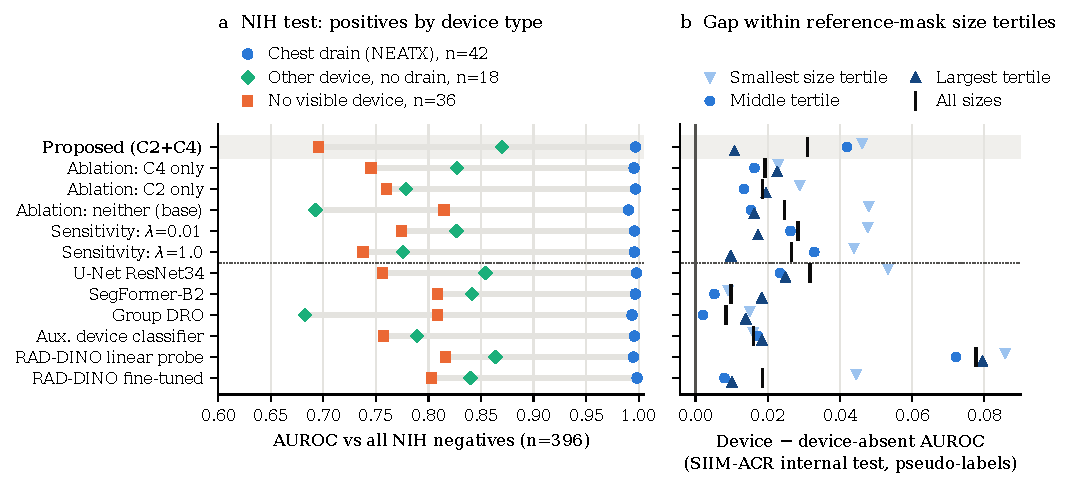
\includegraphics[width=\linewidth]{figures/fig_posthoc_strata.pdf}
\caption{Device type and lesion size (post hoc analyses). (a) NIH test: AUROC of seed-averaged scores for positives with an NEATX-annotated chest drain, positives with another visible device but no drain, and device-absent positives, each against all 396 negatives. (b) SIIM-ACR internal test: device--device-absent AUROC difference within tertiles of reference-mask area and overall (pseudo device labels). The RAD-DINO models have no segmentation output but are scored on the same images.}
\label{fig:strata}
\end{figure*}}{}

\subsection{Patient overlap (post hoc)}
\label{sec:res-overlap}
Excluding the 75 NIH test images of the 46 patients with mapped SIIM-ACR development images removed 52 device-present positives, 17 device-absent positives and 6 negatives, leaving 446 images of 440 patients: 37 device-present and 19 device-absent positives and 390 negatives. \Cref{tab:overlap} reports all main endpoints in this subset. In this subset, device-present AUROC fell for every configuration (proposed model 0.954 to 0.902; base 0.892 to 0.784), indicating that patient overlap had inflated performance on device-present positives. The proposed model's gap remained the largest (0.286, 95\% CI 0.107--0.462). The gap point estimate remained positive for eleven configurations, but it was close to zero for Group DRO (0.006) and slightly negative for base ($-$0.002), and its CI excluded zero for eight configurations; it included zero for the C2-only ablation, SegFormer-B2, base and Group DRO. Device-absent sensitivity at the transferred threshold was 3 of 19 for the proposed model (Wilson 95\% CI 0.06--0.38) and 1 to 4 of 19 for the other configurations, so this endpoint cannot distinguish the models in the subset. The device-in-score AUROC changed little (proposed model 0.703, 95\% CI 0.65--0.76), because only six negatives were removed. In paired comparisons, the proposed model's gap remained larger than those of base and Group DRO after Holm adjustment (both $p_\text{Holm}=0.022$); no other adjusted difference was significant. With only 19 device-absent positives, these estimates are imprecise. The statement that every configuration shows a device-associated gap therefore holds for the pre-specified analysis, but after removal of the identified patient overlap it holds robustly only for eight of the twelve configurations, and not for base or Group DRO. Because the mapping covers only NEATX-annotated images, residual overlap cannot be excluded: the primary test cohort is external with respect to model training but not demonstrably patient-independent of the development data. No second patient-independent external cohort with device annotations and device-absent positives was available to us.

\begin{table*}[!t]
\centering\small
\setlength{\tabcolsep}{3.5pt}
\caption{NIH test set after exclusion of the 75 images of the 46 patients with mapped SIIM-ACR development images (post hoc; 446 images of 440 patients: 37 device-present and 19 device-absent positives, 390 negatives). AUROCs and device-in-score with 95\% patient-cluster bootstrap CIs; device-absent sensitivity at the transferred threshold as detected/total with Wilson 95\% CIs.}
\label{tab:overlap}
\begin{tabular}{@{}l c c c c c@{}}
\toprule
 & \multicolumn{2}{c}{AUROC vs all negatives} & Gap & Device-in- & Sens.\ dev.-abs. \\
\cmidrule(lr){2-3}
Model & Device-absent & Device & (\cref{eq:gap}) & score & (transferred thr.) \\
\midrule
\rowcolor{band}\textbf{Proposed (C2+C4)} & 0.616 \ci{0.44}{0.79} & 0.902 \ci{0.83}{0.95} & 0.286 \ci{0.11}{0.46} & 0.703 \ci{0.65}{0.76} & 3/19 \ci{0.06}{0.38} \\
C4 only & 0.703 \ci{0.56}{0.84} & 0.872 \ci{0.78}{0.94} & 0.169 \ci{0.01}{0.33} & 0.586 \ci{0.53}{0.64} & 4/19 \ci{0.09}{0.43} \\
C2 only & 0.713 \ci{0.59}{0.83} & 0.839 \ci{0.72}{0.92} & 0.126 \ci{$-$0.02}{0.27} & 0.482 \ci{0.42}{0.54} & 4/19 \ci{0.09}{0.43} \\
Base (neither) & 0.786 \ci{0.64}{0.91} & 0.784 \ci{0.66}{0.88} & $-$0.002 \ci{$-$0.17}{0.16} & 0.467 \ci{0.41}{0.53} & 4/19 \ci{0.09}{0.43} \\
$\lambda$=0.01 (C2) & 0.676 \ci{0.52}{0.82} & 0.860 \ci{0.76}{0.93} & 0.184 \ci{0.01}{0.35} & 0.557 \ci{0.49}{0.62} & 3/19 \ci{0.06}{0.38} \\
$\lambda$=1.0 (C2) & 0.641 \ci{0.48}{0.80} & 0.839 \ci{0.72}{0.92} & 0.197 \ci{0.00}{0.39} & 0.541 \ci{0.48}{0.60} & 4/19 \ci{0.09}{0.43} \\
\midrule
U-Net ResNet34 & 0.673 \ci{0.52}{0.82} & 0.902 \ci{0.84}{0.95} & 0.229 \ci{0.07}{0.38} & 0.634 \ci{0.58}{0.69} & 2/19 \ci{0.03}{0.31} \\
SegFormer-B2 & 0.752 \ci{0.63}{0.87} & 0.882 \ci{0.79}{0.95} & 0.130 \ci{$-$0.01}{0.27} & 0.553 \ci{0.49}{0.61} & 4/19 \ci{0.09}{0.43} \\
Group DRO & 0.789 \ci{0.65}{0.91} & 0.795 \ci{0.67}{0.89} & 0.006 \ci{$-$0.17}{0.18} & 0.408 \ci{0.35}{0.47} & 4/19 \ci{0.09}{0.43} \\
Aux.\ device classifier & 0.696 \ci{0.54}{0.84} & 0.864 \ci{0.77}{0.93} & 0.168 \ci{0.00}{0.33} & 0.636 \ci{0.58}{0.69} & 4/19 \ci{0.09}{0.43} \\
RAD-DINO probe & 0.757 \ci{0.62}{0.88} & 0.926 \ci{0.86}{0.96} & 0.169 \ci{0.03}{0.31} & 0.600 \ci{0.54}{0.66} & 1/19 \ci{0.01}{0.25} \\
RAD-DINO fine-tuned & 0.749 \ci{0.61}{0.87} & 0.905 \ci{0.84}{0.95} & 0.156 \ci{0.02}{0.29} & 0.691 \ci{0.64}{0.74} & 3/19 \ci{0.06}{0.38} \\
\bottomrule
\end{tabular}
\end{table*}

\subsection{Location of the top-$k$ decision pixels (post hoc)}
\label{sec:res-topk}
The released checkpoints of the ten segmentation-based configurations were re-run once in inference mode. The re-computed logits matched the stored predictions (maximum absolute difference 0.094 logit units across all 54 runs and three datasets, attributable to half-precision arithmetic on a different GPU; all AUROCs identical). For every positive with a reference mask, \cref{fig:topk} reports the fraction of the $k=1{,}310$ top-scoring pixels of $Z$ that lie inside the mask and within 25~pixels of it, and whether the single highest-scoring pixel lies inside the mask. On the SIIM-ACR internal test set (476 positives), 57--63\% of the top-$k$ pixels lay inside the reference mask and 78--84\% within 25~pixels of it, against 1.4\% expected by chance, and the highest-scoring pixel lay inside the mask in 68--77\% of images. On PTX-498 (482 positives, three hospitals) the corresponding values were 81--91\%, 87--96\% and 84--93\%. The proposed model was in the same range as the other configurations (SIIM-ACR 58.8\%, 80.3\% and 72.3\%; PTX-498 81.4\%, 87.1\% and 84.8\%). Overlap was lower for small lesions (top-$k$ pixels within 25~pixels of the mask: 62--71\% in the smallest and 91--94\% in the largest area tertile) and slightly lower in device-present than in device-absent positives (proposed model 58.3\% versus 62.2\% inside the mask). In pneumothorax-positive images, the score is therefore computed mostly from pixels on or next to the pneumothorax, for every segmentation model. The device-associated differences are consequently not explained by the top-$k$ pixels of positive images falling on devices; they are consistent with device-dependent differences in the magnitude of the pixel logits and with high-scoring responses in negatives, which have no reference region and could not be localised in this analysis (\cref{sec:res-shortcut,sec:res-qual}).

\IfFileExists{figures/fig_posthoc_topk.pdf}{%
\begin{figure*}[!t]
\centering
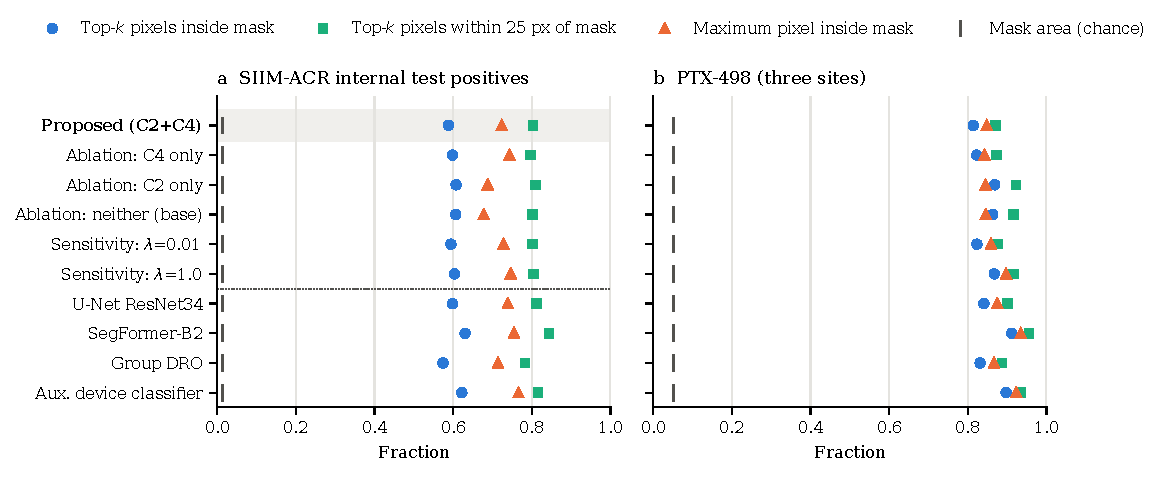
\includegraphics[width=\linewidth]{figures/fig_posthoc_topk.pdf}
\caption{Overlap of the top-$k$ decision pixels ($k=1{,}310$) with the reference pneumothorax mask for the ten segmentation-based configurations, averaged over positive images and seeds. (a) SIIM-ACR internal test (476 positives). (b) PTX-498 (482 positives). Vertical ticks: mask area as a fraction of the image (the overlap expected by chance).}
\label{fig:topk}
\end{figure*}}{}

\subsection{Training dynamics}
\label{sec:res-conv}
\Cref{fig:convergence} shows per-epoch training and validation curves (mean and min--max over seeds). Training classification loss fell steadily to $10^{-2}$--$10^{-3}$ for the EfficientNet-B4 variants and the fine-tuned RAD-DINO, while validation AUROC reached 0.93--0.96, mostly within the first few epochs, and changed little afterwards (Group DRO declined to 0.91). Validation device-absent sensitivity on SIIM-ACR reached 0.72--0.79 for the EfficientNet-B4 variants and 0.79 for SegFormer-B2, far above the 0.08--0.31 per-seed values observed at the same thresholds on NIH (\cref{fig:seeds}). Its min--max band was wide, reflecting the 32 device-absent validation positives, and the epoch selected by \cref{line:select} of \cref{alg:train} varied from 3 to 15 (of 20) across the proposed model's seeds. Validation Dice peaked early (about 0.50--0.54) and then drifted down slightly.

\textbf{Stability of checkpoint selection (post hoc).} Across the 54 runs, the selection rule chose epochs 2 to 18. The criterion is coarse: in 20 runs (37\%) the maximum validation device-absent sensitivity was reached at more than one epoch and the first was kept, and a median of three epochs (range 1--11) lay within one validation case (1/32) of the maximum, so that a change in the classification of a single case could have moved the selected epoch. Selection by validation AUROC would have chosen the same epoch in only 3 of 54 runs, at a median cost of 0.008 (maximum 0.036) in validation AUROC for the epoch that was kept. Across runs, the selected validation value correlated with device-absent sensitivity on NIH (Spearman $\rho=0.52$), mainly because configurations differed (the RAD-DINO linear probe was low on both); within configurations the correlation ranged from $-$0.87 to 0.92 without a consistent sign, and across runs it was not associated with NIH device-absent AUROC ($\rho=-0.25$, $p=0.07$). Selection on 32 device-absent validation positives was therefore unstable and did not identify checkpoints that generalised better on this stratum. Only the selected checkpoint of each run was retained, so the external performance of other epochs could not be evaluated.

The training dynamics of the device head differed from those intended in the design (\cref{fig:auxloss}b). In the proposed model the adversary's loss fell from 0.88 to 0.61 within three epochs and then stayed at the chance level of 0.60 (the label entropy for a batch device prevalence of about 0.71 under 50\% positive sampling). The encoder had therefore made $h$ uninformative \emph{to the adversary} on the development data. With the global head, adversarial losses stayed below chance for $\lambda=0.01$ (0.55) and $\lambda=0.1$ (0.58) and reached it only for $\lambda=1$. Without gradient reversal, the auxiliary device classifier drove its loss to nearly zero, confirming that device status is easy to read from the same features. Yet on NIH, device information remained linearly recoverable from the proposed model's $h$ (probe AUROC 0.900), and its score carried the strongest device signal of all models (device-in-score 0.710).

\begin{figure*}[!t]
\centering
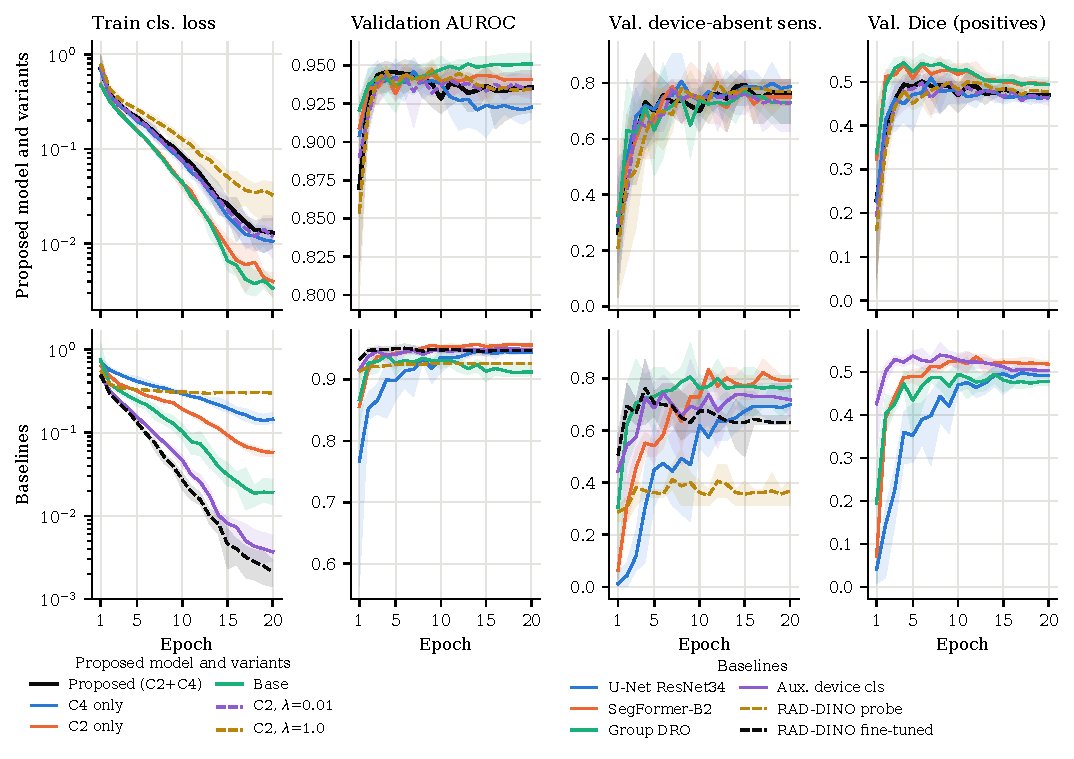
\includegraphics[width=\linewidth]{figures/fig_convergence.pdf}
\caption{Convergence curves on SIIM-ACR (mean with min--max band over 3--5 seeds). Top: proposed model, ablations and sensitivity variants; bottom: baselines. Training classification loss is on a log scale. Validation device-absent sensitivity is computed at each epoch's own 95\%-specificity threshold on 32 device-absent validation positives; it is the checkpoint-selection criterion of \cref{alg:train}. RAD-DINO models have no segmentation output.}
\label{fig:convergence}
\end{figure*}

\begin{figure*}[!t]
\centering
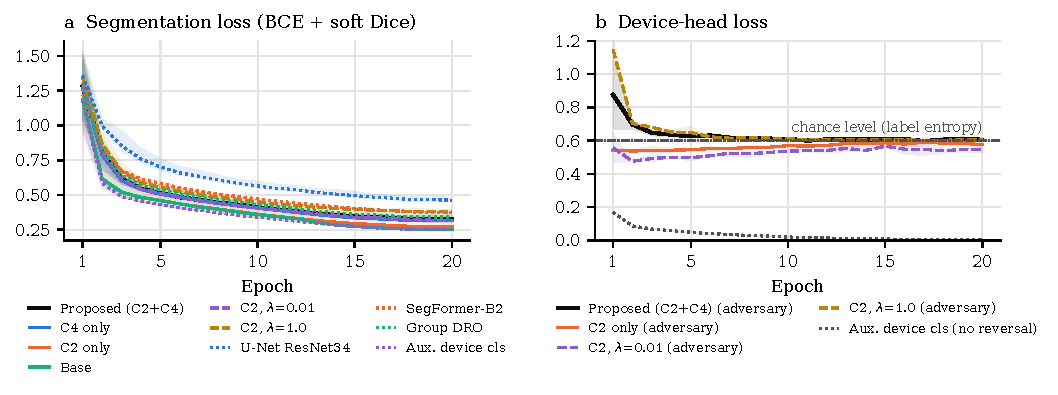
\includegraphics[width=\linewidth]{figures/fig_aux_losses.pdf}
\caption{Auxiliary training losses (mean with min--max band). (a) Segmentation loss (\cref{eq:lseg}); dotted lines are baselines. (b) Device-head loss: the adversary of \cref{eq:ladv} for C2 variants, and the auxiliary device classifier without reversal (logged with its loss weight 0.5). The dash-dotted line is the chance level, the entropy of the device label in training batches.}
\label{fig:auxloss}
\end{figure*}

\subsection{Ablations and sensitivity runs}
\label{sec:res-ablation}
Neither component improved device-absent sensitivity (\cref{tab:ablation}). The values in \cref{tab:ablation} are means of per-seed sensitivities, each at the seed's own threshold, whereas \cref{tab:nih,tab:endpoints} use seed-averaged scores and one threshold; for the proposed model the two conventions give 0.206 and 0.222. Removing the adversary (C4 only) \emph{raised} mean per-seed device-absent sensitivity from 0.206 to 0.256 and lowered the AUC gap from 0.258 to 0.191. Removing both components (base) gave the second-smallest gap of all models (0.077) and one of the highest device-absent AUROCs (0.815). Among the C2 variants with a global head, $\lambda$ did not produce a monotone improvement (gap 0.159, 0.159 and 0.172 for $\lambda$ = 0.01, 0.1 and 1.0).

\begin{table*}[!t]
\centering\small
\caption{Ablations on the NIH test set. ``Full'' and ``Ablated'' are device-absent sensitivities averaged over 5 seeds, each seed scored at its own transferred threshold (mean of per-seed values; 0.206 for the proposed model, against 0.222 from seed-averaged scores in \cref{tab:nih}); ``seeds with drop'' counts paired seeds in which removing the component lowered the metric. Difference = full minus ablated, computed from seed-averaged scores with 95\% patient-cluster bootstrap CIs.}
\label{tab:ablation}
\begin{tabular}{@{}l l c c c c@{}}
\toprule
Ablation & Removed & Full & Ablated & Seeds with drop & Diff.\ (seed-avg) \ci{95\%}{CI} \\
\midrule
C4 only & C2 adversary & 0.206 & 0.256 & 1/5 & $-$0.028 \ci{$-$0.095}{0.000} \\
C2 only & C4 mask pooling & 0.206 & 0.211 & 2/5 & $-$0.056 \ci{$-$0.147}{0.000} \\
Base & C2 and C4 & 0.206 & 0.206 & 3/5 & $-$0.028 \ci{$-$0.095}{0.000} \\
\bottomrule
\end{tabular}
\end{table*}

\subsection{The device-associated difference across architectures (exploratory)}
\label{sec:res-shortcut}
In the pre-specified analysis, every configuration detected device-present pneumothorax better than device-absent pneumothorax (\cref{fig:shortcut}a; \cref{tab:nih}); after exclusion of the identified patient overlap this remained clear for eight configurations (\cref{sec:res-overlap}). Point estimates of the gap ranged from 0.077 (base) to 0.258 (proposed). The gap's CI excluded zero for ten of twelve configurations; the exceptions were base and Group DRO. The radiology foundation model showed the same pattern: RAD-DINO had the highest overall AUROC (0.916), yet its gap was 0.140 when frozen and 0.148 when fine-tuned.

The score-level analysis (\cref{fig:shortcut}c) is consistent with a device association in the score itself. Among pneumothorax-negative NIH radiographs, device-bearing images scored higher than device-free images in eight of twelve configurations (\cref{eq:devscore} between 0.56 and 0.71, CI excluding 0.5). The proposed model had the strongest effect (0.710, 95\% CI 0.66--0.76). The configurations without this effect were base (0.477), Group DRO (0.416), C2 only (0.491) and the $\lambda$=1.0 variant (0.545, CI including 0.5). Stratification by projection (\cref{sec:res-strata}) shows that the pooled values of base, Group DRO and C2 only were influenced by the higher proportion of AP radiographs among device-bearing negatives: within PA radiographs, the device-in-score point estimate exceeded 0.5 for all twelve configurations (CI excluding 0.5 for eight).

In paired comparisons (\cref{fig:paired}), the 95\% CI of the difference in device-absent AUROC excluded zero against base, Group DRO, SegFormer-B2, both RAD-DINO models and the $\lambda$=0.01 variant, and the CI of the difference in gap excluded zero against seven of eleven comparators. After Holm adjustment for the eleven comparisons, the device-absent AUROC was significantly lower only than that of the RAD-DINO linear probe, and the gap was significantly larger only than those of base, Group DRO and the RAD-DINO linear probe; the remaining differences are nominal. These tests treat the trained models as fixed. When variation between training seeds is included (\cref{sec:res-seeds}), none of these differences remains significant after adjustment.

\begin{figure*}[!t]
\centering
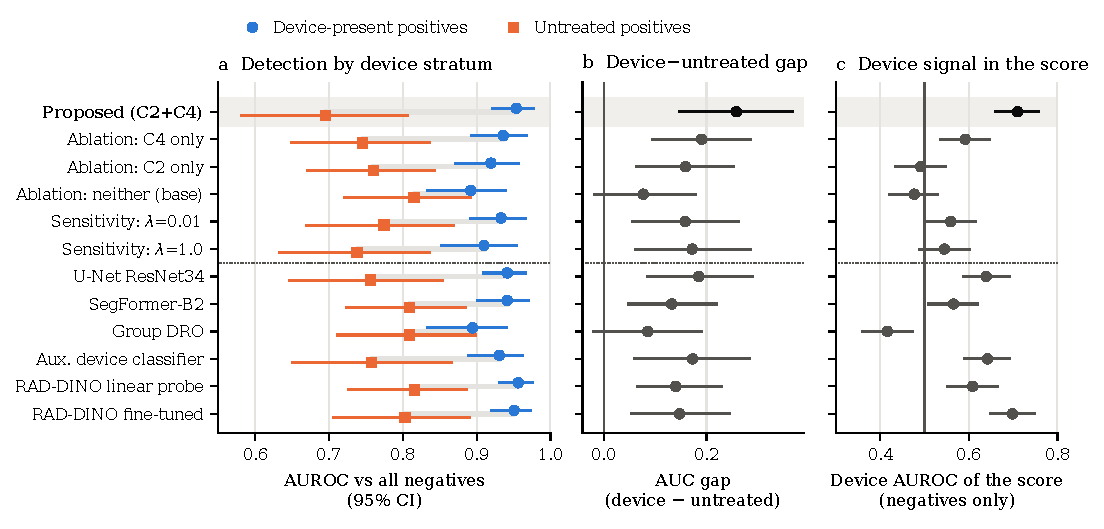
\includegraphics[width=\linewidth]{figures/fig2_shortcut.pdf}
\caption{Device shortcut on the NIH test set (seed-averaged scores; 95\% patient-cluster bootstrap CIs). (a) AUROC for device-present versus device-absent pneumothorax against all negatives. (b) The gap between them (\cref{eq:gap}; primary endpoint). (c) Device AUROC of the pneumothorax score among pneumothorax-negative images (\cref{eq:devscore}); values above 0.5 mean that device-bearing negatives score higher than device-free negatives. The dotted line separates the proposed model and its variants from the baselines.}
\label{fig:shortcut}
\end{figure*}

\begin{figure*}[!t]
\centering
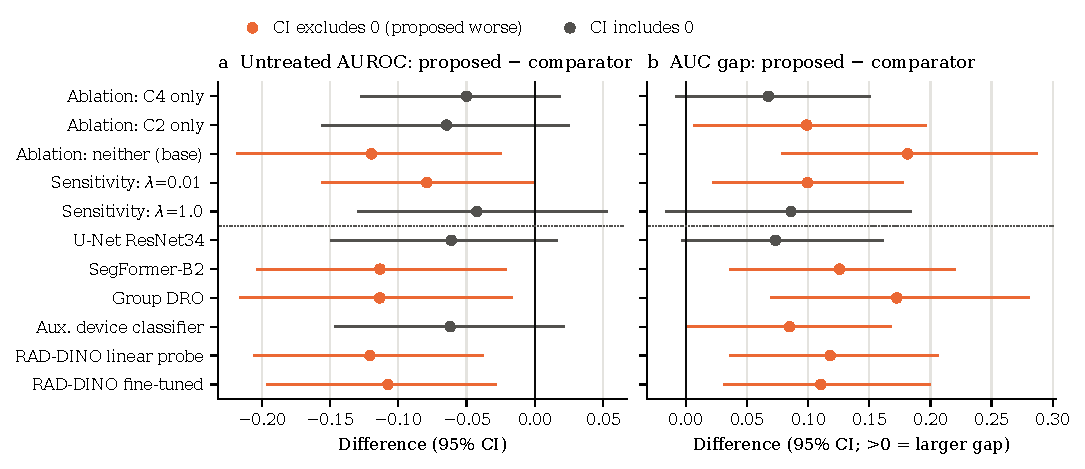
\includegraphics[width=\linewidth]{figures/fig3_paired.pdf}
\caption{Paired bootstrap differences between the proposed model and each comparator on the NIH test set (exploratory; shared patient resamples, \cref{alg:boot}; trained models treated as fixed, see \cref{tab:seeds} for intervals that include seed variation). Orange marks CIs that exclude zero in the direction unfavourable to the proposed model.}
\label{fig:paired}
\end{figure*}

\begin{figure*}[!t]
\centering
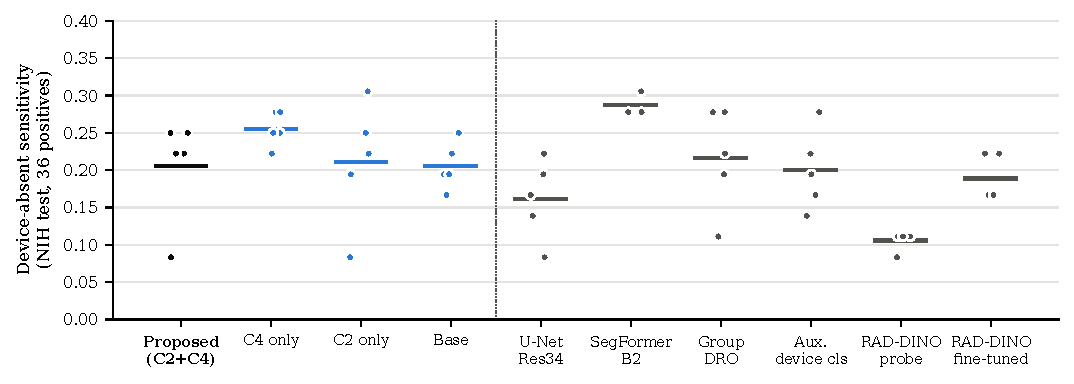
\includegraphics[width=\linewidth]{figures/fig4_seeds.pdf}
\caption{Per-seed device-absent sensitivity on the NIH test set at the threshold transferred from SIIM-ACR validation (36 device-absent positives, so one case = 0.028). Bars show seed means.}
\label{fig:seeds}
\end{figure*}

\subsection{Variation between training seeds (post hoc)}
\label{sec:res-seeds}
\Cref{tab:seeds} reports, for every configuration, the mean and standard deviation over seeds of the NIH endpoints computed per seed, and CIs for the seed-averaged estimates from the two-stage bootstrap over patients and seeds (\cref{sec:stats}). Seed-to-seed variation was substantial for the EfficientNet-B4 variants: the proposed model's device-absent AUROC ranged from 0.57 to 0.75 and its gap from 0.15 to 0.37 across seeds, whereas the device-absent AUROC and gap of the RAD-DINO linear probe each varied by less than 0.03. Including seed variation widened the CI of the proposed model's gap from 0.15--0.37 to 0.12--0.43. The gap CI excluded zero for ten configurations and included zero for base and Group DRO, as in the patient-only analysis. For paired comparisons the effect was larger: none of the eleven differences between the proposed model and the other configurations in device-absent AUROC, gap or device-absent sensitivity remained significant after Holm adjustment. Without adjustment, the CI excluded zero only for the gap relative to Group DRO (difference 0.173, 95\% CI 0.018--0.327) and for the device-absent AUROC relative to the RAD-DINO linear probe ($-$0.121, $-$0.277 to $-$0.009). At the level of individual runs, each of the five proposed-model seeds had a larger gap (0.15--0.37) than each of the five Group DRO seeds (0.05--0.15). The patient-level comparisons in \cref{sec:res-shortcut} are therefore conditional on the trained models: the larger gap of the proposed model is consistent across seeds and point estimates, but it is not supported by a multiplicity-adjusted test that accounts for training variability.

\begin{table*}[!t]
\centering\footnotesize
\setlength{\tabcolsep}{2.5pt}
\caption{Variation between training seeds on the NIH test set (post hoc). Left: per-seed endpoints (each seed scored with its own transferred threshold), mean $\pm$ standard deviation over seeds, with the range of the gap. Right: seed-averaged estimates with 95\% CIs from the two-stage bootstrap over patients and seeds.}
\label{tab:seeds}
\begin{tabular}{@{}l c c c c c c c@{}}
\toprule
 & & \multicolumn{4}{c}{Per seed (mean $\pm$ SD)} & \multicolumn{2}{c}{Seed-averaged, two-stage CI} \\
\cmidrule(lr){3-6}\cmidrule(l){7-8}
Model & Seeds & AUROC dev.-abs. & Gap (range) & Device-in-score & Sens.\ dev.-abs. & AUROC dev.-abs. & Gap \\
\midrule
\rowcolor{band}\textbf{Proposed (C2+C4)} & 5 & 0.676 $\pm$ 0.078 & 0.244 $\pm$ 0.081 (0.15--0.37) & 0.625 $\pm$ 0.054 & 0.205 $\pm$ 0.070 & 0.695 \ci{0.52}{0.82} & 0.258 \ci{0.12}{0.43} \\
C4 only & 5 & 0.691 $\pm$ 0.069 & 0.205 $\pm$ 0.061 (0.13--0.27) & 0.557 $\pm$ 0.036 & 0.256 $\pm$ 0.023 & 0.745 \ci{0.60}{0.84} & 0.191 \ci{0.08}{0.33} \\
C2 only & 5 & 0.739 $\pm$ 0.024 & 0.154 $\pm$ 0.030 (0.11--0.18) & 0.462 $\pm$ 0.056 & 0.211 $\pm$ 0.082 & 0.760 \ci{0.65}{0.85} & 0.159 \ci{0.04}{0.26} \\
Base (neither) & 5 & 0.734 $\pm$ 0.054 & 0.162 $\pm$ 0.060 (0.07--0.22) & 0.532 $\pm$ 0.062 & 0.205 $\pm$ 0.032 & 0.815 \ci{0.66}{0.89} & 0.077 \ci{$-$0.01}{0.25} \\
$\lambda$=0.01 (C2) & 3 & 0.726 $\pm$ 0.064 & 0.182 $\pm$ 0.066 (0.11--0.24) & 0.471 $\pm$ 0.118 & 0.195 $\pm$ 0.048 & 0.774 \ci{0.61}{0.86} & 0.159 \ci{0.04}{0.32} \\
$\lambda$=1.0 (C2) & 3 & 0.716 $\pm$ 0.019 & 0.180 $\pm$ 0.026 (0.15--0.20) & 0.549 $\pm$ 0.043 & 0.250 $\pm$ 0.048 & 0.738 \ci{0.62}{0.83} & 0.172 \ci{0.05}{0.29} \\
\midrule
U-Net ResNet34 & 5 & 0.716 $\pm$ 0.042 & 0.206 $\pm$ 0.046 (0.16--0.28) & 0.629 $\pm$ 0.029 & 0.161 $\pm$ 0.053 & 0.756 \ci{0.62}{0.84} & 0.185 \ci{0.09}{0.31} \\
SegFormer-B2 & 3 & 0.795 $\pm$ 0.017 & 0.134 $\pm$ 0.017 (0.12--0.15) & 0.556 $\pm$ 0.034 & 0.287 $\pm$ 0.016 & 0.809 \ci{0.71}{0.88} & 0.133 \ci{0.05}{0.23} \\
Group DRO & 5 & 0.774 $\pm$ 0.038 & 0.096 $\pm$ 0.040 (0.05--0.15) & 0.434 $\pm$ 0.079 & 0.217 $\pm$ 0.069 & 0.809 \ci{0.68}{0.89} & 0.086 \ci{$-$0.02}{0.22} \\
Aux.\ device classifier & 5 & 0.718 $\pm$ 0.048 & 0.203 $\pm$ 0.050 (0.15--0.29) & 0.645 $\pm$ 0.106 & 0.200 $\pm$ 0.053 & 0.757 \ci{0.63}{0.85} & 0.173 \ci{0.07}{0.31} \\
RAD-DINO probe & 5 & 0.814 $\pm$ 0.011 & 0.141 $\pm$ 0.011 (0.13--0.16) & 0.607 $\pm$ 0.007 & 0.105 $\pm$ 0.012 & 0.816 \ci{0.72}{0.89} & 0.140 \ci{0.06}{0.23} \\
RAD-DINO fine-tuned & 5 & 0.798 $\pm$ 0.022 & 0.149 $\pm$ 0.020 (0.12--0.17) & 0.667 $\pm$ 0.076 & 0.189 $\pm$ 0.030 & 0.803 \ci{0.70}{0.89} & 0.148 \ci{0.06}{0.25} \\
\bottomrule
\end{tabular}
\end{table*}

\subsection{Operating-point transfer (exploratory)}
\label{sec:res-threshold}
Thresholds set at 95\% specificity on SIIM-ACR validation reproduced the intended operating point on the SIIM-ACR internal test set (specificity 0.940--0.963) but were far too strict on NIH: specificity was 0.992--1.000 for every model, and overall sensitivity only 0.40--0.49. The shift was not explained by the lower device prevalence among NIH negatives (39.8\% versus 55.3\% in SIIM-ACR validation): specificity was 0.981--1.000 among device-bearing and 0.996--1.000 among device-free NIH negatives. It was explained by a shift of the whole score distribution (\cref{fig:threshold}). The 95th percentile of negative scores fell from 0.52--0.84 on SIIM-ACR validation to 0.02--0.37 on NIH (Kolmogorov--Smirnov distance between the negative logit distributions 0.19--0.31), and positive scores fell as well (median 0.80--0.95 on the SIIM-ACR internal test versus 0.38--0.77 on NIH; for device-absent positives 0.62--0.95 versus 0.005--0.24). The NIH negatives are radiographs labelled ``no finding'', whereas SIIM-ACR negatives include radiographs with other abnormalities; a difference in case mix, with easier negatives and less conspicuous positives, is the most likely cause, but the data cannot attribute the shift to a single factor. With a threshold recalibrated at 95\% specificity on the NIH set itself (an oracle, not a valid clinical estimate), overall sensitivity rose to 0.65--0.75 and device-absent sensitivity to 0.36--0.58. The proposed model reached 0.744 overall and 0.444 device-absent; the fine-tuned RAD-DINO model had the highest device-absent value (0.583). Device-absent sensitivity was therefore low in every model at every threshold considered, and the threshold-independent stratified AUROCs (\cref{tab:nih}) are the more informative comparison between models.

\IfFileExists{figures/fig_posthoc_threshold.pdf}{%
\begin{figure*}[!t]
\centering
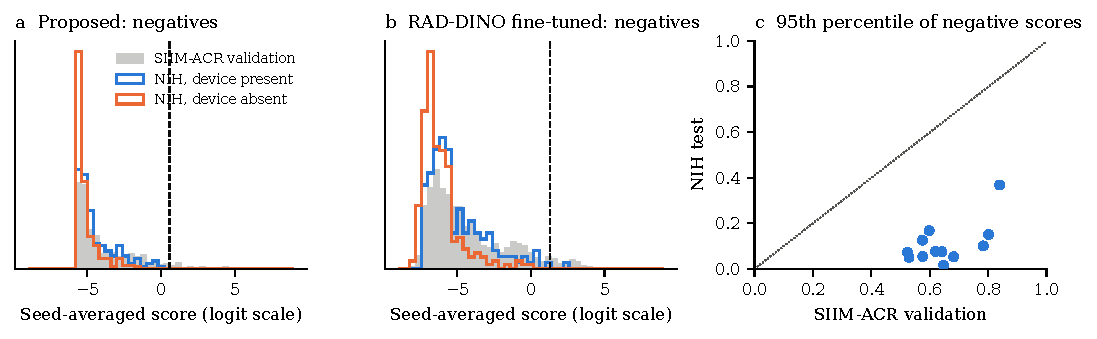
\includegraphics[width=\linewidth]{figures/fig_posthoc_threshold.pdf}
\caption{Threshold transfer (post hoc analysis). (a, b) Distributions of seed-averaged scores of negatives on SIIM-ACR validation and of device-bearing and device-free negatives on the NIH test set, for the proposed model and the fine-tuned RAD-DINO model; the dashed line is the threshold set at 95\% specificity on SIIM-ACR validation. (c) 95th percentile of negative scores on SIIM-ACR validation and on NIH for all twelve configurations; the dotted line is identity.}
\label{fig:threshold}
\end{figure*}}{}

\subsection{Example images and model maps (exploratory)}
\label{sec:res-qual}
Examples were chosen by rules fixed in the rendering script before any image was viewed, using the proposed model's seed-averaged NIH scores: the device-absent positive with the highest score (device-absent TP), the device-absent positive with the lowest score (device-absent FN), the device-present positive with the median score, the device-present \emph{negative} with the highest score (a candidate for device-associated bias), and a device-free negative with the median score; plus two random SIIM-ACR internal-test positives with masks and one random PTX-498 image per site (random seed 0). For each model we averaged over seeds the segmentation probability $\sigma(Z)$ and Grad-CAM \cite{selvaraju2020gradcam} of the image logit $s(x)$ on the last encoder stage.

\Cref{fig:examples} shows the selected images and \cref{fig:maps} the seed-averaged maps for five models. The device-absent positive with the highest score has a visible apical pneumothorax, and every model segmented it and scored it high (seed-averaged probability 0.86--1.00). The device-absent positive with the lowest score is a device-free film on which the pneumothorax is not apparent at figure resolution; every model missed it (probability $\le$0.09), with no segmentation response and diffuse Grad-CAM. In the device-bearing \emph{negative} with the highest proposed-model score, several lines and ECG leads cross the chest. The proposed model, C4 only, SegFormer-B2 and Group DRO all placed pneumothorax probability over an upper zone crossed by these lines (probabilities 0.37--0.87), whereas the base model responded weakly (0.20). This single case matches the score-level result (\cref{eq:devscore}): in this example the mask-pooling models assign pneumothorax probability to device-related structures, and the global-head base model does so least. It is an illustration, not evidence; the quantitative test is \cref{tab:nih}.

\IfFileExists{figures/fig_examples.pdf}{%
\begin{figure*}[!t]
\centering
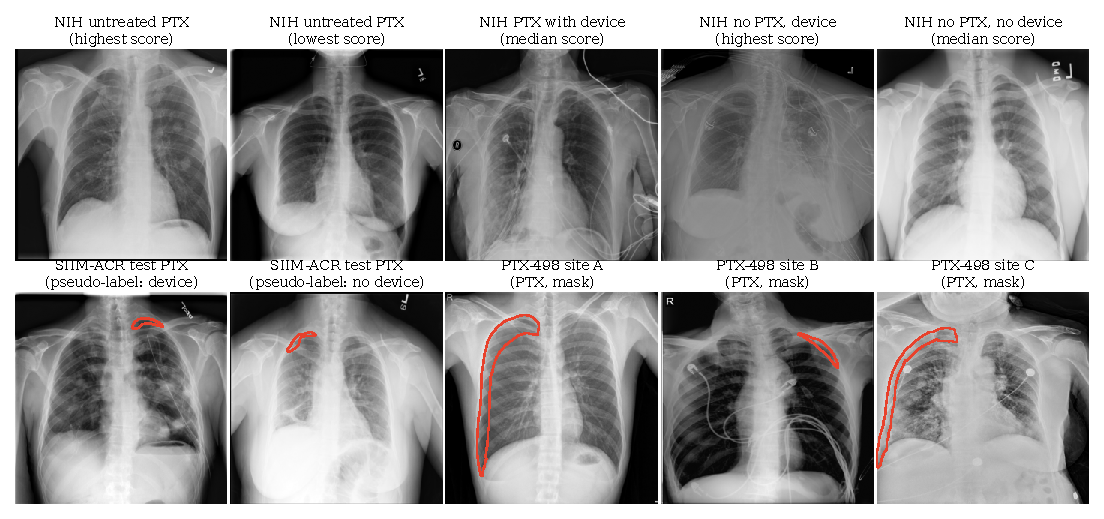
\includegraphics[width=\linewidth]{figures/fig_examples.pdf}
\caption{Example radiographs from each dataset with reference pneumothorax masks where available (red outline). NIH images are labelled with the human device annotation. Examples were chosen by fixed rules (\cref{sec:res-qual}).}
\label{fig:examples}
\end{figure*}}{}

\IfFileExists{figures/fig_maps.pdf}{%
\begin{figure*}[!t]
\centering
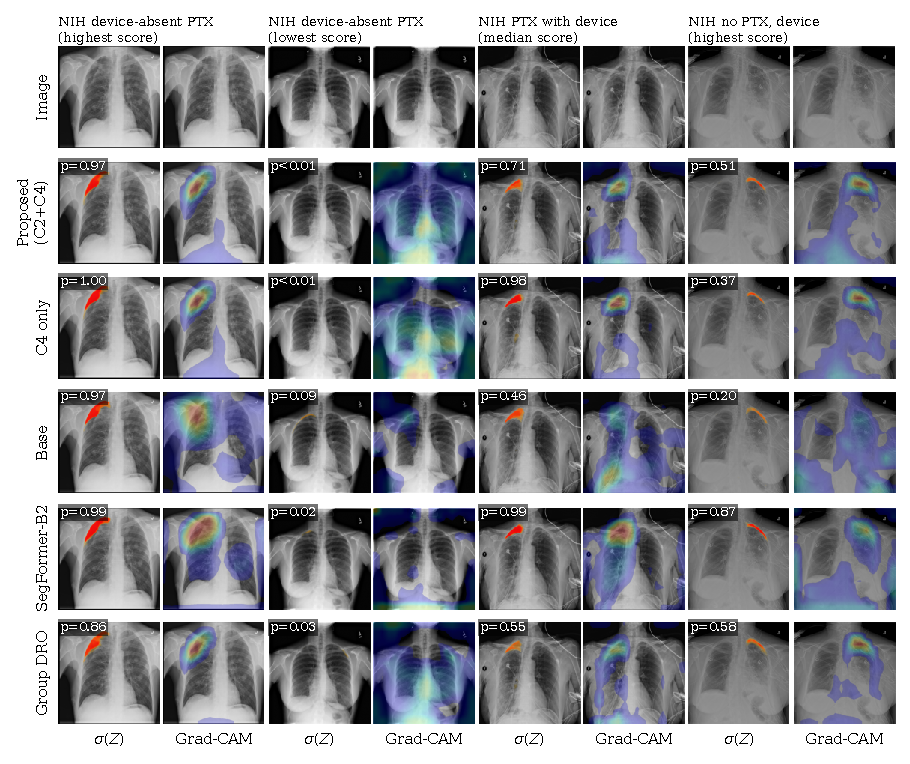
\includegraphics[width=\linewidth]{figures/fig_maps.pdf}
\caption{Seed-averaged model maps on the four NIH test cases selected by fixed rules. For each case, the left column shows the pneumothorax probability map $\sigma(Z)$ (red, opacity proportional to probability) and the right column Grad-CAM of the image logit $s(x)$. Numbers are seed-averaged predicted probabilities. Rows are models; the base model uses the global head, so its score does not depend on $\sigma(Z)$. Maps are illustrations only (see \cref{sec:discussion}).}
\label{fig:maps}
\end{figure*}}{}


%% ============================================================ DISCUSSION
\section{Discussion}
\label{sec:discussion}

The hypothesis was not supported. A U-Net with a gradient-reversal device adversary and segmentation-based mask pooling, trained on SIIM-ACR with device pseudo-labels, did not detect device-absent pneumothorax better than the baselines on external data, and it had the largest device--device-absent gap of the twelve configurations. The evidence differs in strength between endpoints. For device-absent sensitivity at the transferred threshold, the comparison with the best baseline rests on two cases and its CI reaches zero, so the result is a failure to show superiority rather than a demonstration of inferiority; the proposed model detected more device-absent cases than three baselines (U-Net ResNet34, both RAD-DINO models). For the threshold-independent quantities, the proposed model had the largest gap and the lowest device-absent AUROC point estimates of the twelve configurations. Conditional on the trained models, its gap exceeded those of base, Group DRO and the RAD-DINO linear probe after Holm adjustment, and its device-absent AUROC was below that of the RAD-DINO linear probe (pre-specified DeLong test, $p_\text{Holm}=0.046$; clustered, 0.023). When variation between training seeds is included, these differences are not significant after adjustment, although each seed of the proposed model had a larger gap than each Group DRO seed (\cref{sec:res-seeds}). The study therefore shows that adversarial deconfounding, as implemented here, did not reduce the device-associated gap; it does not establish with an adjusted test that it increased it.

\paragraph{Why the deconfounding failed}
Several explanations are consistent with the data; the design cannot fully separate them.
\begin{enumerate}
  \item \emph{The adversary constrained the wrong pathway.} The adversary acted on globally pooled encoder features $h$, whereas C4 computes the decision from the decoder's segmentation logits $Z$ (\cref{fig:arch}). The training curves show that the adversary was driven to chance (\cref{fig:auxloss}b), so on the development data $h$ was uninformative to that particular head. The segmentation pathway, which bypasses $h$ through skip connections, was unconstrained. The top-$k$ analysis (\cref{sec:res-topk}) refines this point: in positives the decision pixels lay mostly on the lesion, so the misalignment does not lie in where the score is read but in which features determine the magnitude of the pixel logits there and in negatives, and those features reach the decoder through the unconstrained skip connections. Consistent with this, C2 with a global head (whose score \emph{is} a function of $h$) had a device-in-score AUROC near 0.5, whereas C2 with C4 had the highest value observed. An adversary at chance is therefore not evidence of invariance: a linear probe on the same features still recovered device status externally (AUROC 0.900). Four properties of adversarial training explain why the two observations are compatible. (a) The adversary's loss measures only what the current adversary, with its current weights, can extract; in the min--max game the encoder can make $h$ uninformative to that adversary by moving device information to directions the adversary has not yet learned to read, without removing it. (b) Chance-level loss is measured on training mini-batches with the pseudo-labels, whereas the probe is fitted afresh on held-out data with human labels and is free to find any linear direction. (c) Gradient reversal penalises only information in $h$; information carried through the skip connections to the decoder, from which the mask-pooled score is computed, is not penalised at all. (d) Invariance learned on the development distribution need not transfer to a shifted external distribution. On the SIIM-ACR internal test set, that is, on the development distribution, a linear probe on $h$ still predicted the pseudo-labelled device status with AUROC 0.945 for the proposed model, against 0.957 for base, and predicted annotated chest drains with AUROC 0.897 (base 0.917). The adversary therefore reduced the linearly decodable device information in $h$ only marginally even in distribution, so reasons (a)--(c) are sufficient to account for the observation without distribution shift. A held-out probe, not the adversary's loss, is therefore the appropriate check of removal. This echoes benchmark findings that latent-space analyses reveal differences that task metrics miss \cite{muller2026disentangle}.
  \item \emph{Proxy mismatch.} The adversary targeted ``any visible device'' predicted by a classifier, not the chest drain. The comparison with chest-drain annotations (\cref{sec:res-pseudo}) shows that drains were almost always included in the pseudo-label (97.9\%), so the failure is unlikely to stem from drains being missed. Instead, the attribute was broad: about four in ten pseudo-labelled device-bearing images had no drain, and lines and leads are common in negatives (55\% of SIIM-ACR negatives were labelled device-bearing). Removing ``device'' information is therefore not the same as removing ``drain'' information, and the adversary may have penalised features that are unrelated to the confounder while leaving drain-specific features in the decoder pathway. Worst-group performance with inferred groups is known to trail that with oracle groups \cite{han2024gic,liu2021jtt}. The design cannot separate this explanation from the pathway mismatch in item 1; both are compatible with the data.
  \item \emph{Noisy model selection.} Checkpoints were selected on device-absent sensitivity in a validation set with only 32 device-absent positives, where one case moves the metric by 3 percentage points. The selected epochs ranged from 3 to 15 across the proposed model's seeds, a median of three epochs per run lay within one case of the selected maximum, and the selected validation value did not predict external device-absent discrimination (\cref{sec:res-conv}); a validation value of about 0.76 fell to about 0.2 externally. The validation set also shares patients with the training set (\cref{sec:dependencies}), which favours epochs that fit patient-specific appearance. The pilot's apparent advantage for C2+C4 on this criterion did not replicate.
\end{enumerate}
\paragraph{Scope of the negative result}
The negative result concerns one implementation: a two-layer adversary on the globally pooled deepest encoder features, a mask-pooled decision computed from decoder logits that receive unconstrained skip connections, and a broad, pseudo-labelled device attribute. It does not show that gradient reversal is ineffective for reducing device-associated bias in general. Variants that apply the adversary to decoder features or to the segmentation logits, use adversaries at several depths, penalise the dependence of the image score on device status among negatives, or target an attribute that matches chest drains were not tested and could behave differently.

Simple baselines without attribute-specific machinery (base, Group DRO) had the smallest gaps and, in the pooled analysis, near-chance device-in-score values; within PA radiographs their device-in-score values also exceeded 0.5 (\cref{sec:res-strata}). Removing a shortcut in one distribution does not guarantee better behaviour in another \cite{yang2024limits}, and here the more elaborate debiasing was associated with a larger external gap.

\paragraph{Device-associated differences across architectures}
Across convolutional, transformer and foundation-model backbones, every model detected device-present pneumothorax better than device-absent pneumothorax in the pre-specified analysis (eight of twelve robustly after removal of the identified patient overlap), and in most the score itself was higher for device-bearing negatives. This agrees with reports that thoracic tubes confound pneumothorax algorithms \cite{rueckel2020tubes,rueckel2021annotations}, with saliency evidence of tube bias \cite{wollek2023attention}, with the lower performance of CLIP-based models on drain-free images \cite{sourget2025clip}, and with foundation encoders using tube shortcuts \cite{li2025featurequality}. It contrasts with studies that found no tube effect \cite{thian2021external,seah2021hidden,graf2020tube}. Those models were trained on larger or differently labelled data, used lung segmentation, or tested tube-bearing \emph{positives} against all negatives; the stratum that separates the hypotheses, device-bearing negatives, was rarely analysed. Our device-in-score metric (\cref{eq:devscore}) isolates that stratum and requires only device labels on the test set. Overall AUROC does not reveal the difference: RAD-DINO had the highest overall AUROC and a clear gap.

\paragraph{Association and causation}
The stratified metrics establish device-associated prediction differences; they do not by themselves establish that the models use device pixels. Device-present and device-absent positives can differ in severity, projection, acquisition setting and clinical context. Four analyses address these alternatives; none excludes them. First, among negatives, where there is no disease severity to differ, device-bearing negatives scored higher in eight of twelve configurations overall, and within PA radiographs the point estimate pointed in the same direction for all twelve (CI excluding no difference for eight). Second, within reference-mask size tertiles on SIIM-ACR the difference persisted, and adjustment for lesion area left the device coefficient almost unchanged (\cref{sec:res-strata}). Third, NIH positives with chest drains were detected almost perfectly by every configuration, and for most configurations positives with other devices were detected less well and device-absent positives worst, a gradient consistent with the visual salience of the device type (for base, Group DRO, C2 only and the $\lambda$=1.0 variant, positives with other devices scored lowest). The device--device-absent difference persisted within PA radiographs and after adjustment for projection, sex and age on NIH. Fourth, the seed-averaged mask-pooled maps place high-scoring pixels over device-related structures in device-bearing negatives (\cref{sec:res-qual}), although maps are illustrations only. A causal test would require intervening on device pixels, for example by removing or inserting devices with validated inpainting or counterfactual editing \cite{cooke2026roentmod}, which needs device masks that were not available; we therefore describe the findings as device-associated bias consistent with, but not proof of, shortcut reliance.

\paragraph{Shared development data}
All configurations share the development data, its pseudo-labels, its device prevalence (86.9\% of SIIM-ACR positives were labelled device-bearing versus 55.3\% of negatives), the input resolution, the positive oversampling and the checkpoint-selection rule. The similarity of the results therefore reflects these shared factors at least as much as the architectures. Two observations support this reading. Scores on the 36 NIH device-absent positives were strongly rank-correlated across the twelve configurations (median Spearman correlation 0.86, range 0.66--0.92), and 25 of the 36 were missed by all twelve configurations at their transferred thresholds. The finding that every configuration shows a gap should accordingly be read as a property of models trained on SIIM-ACR with this recipe, not as a property of the architectures in general; models trained on data with a different device--label association could behave differently.

\paragraph{Internal estimates and model selection}
Because 83\% of the mapped SIIM-ACR internal-test images share a patient with training or validation images, the internal-test results (\cref{tab:secondary}) measure in-distribution performance under patient overlap and are not evidence of generalisation; external evidence in this study comes from the NIH test set alone, with PTX-498 limited to sensitivity and segmentation. The same dependence affects model selection. Validation images of training patients favour checkpoints that fit patient-specific appearance, which is consistent with validation device-absent sensitivities of 0.72--0.79 against 0.08--0.31 per seed on NIH, and thresholds placed on validation negatives that resemble training images can be expected to differ from those appropriate for unseen patients. The external estimates do not depend on the internal-test results, but the checkpoints and thresholds on which they rest carry this dependence.

\paragraph{What the heatmaps can and cannot show}
The qualitative maps in \cref{sec:res-qual} are illustrations chosen by fixed rules, not evidence. Saliency methods localise poorly on chest radiographs and can fail sanity checks \cite{saporta2022saliency,arun2021saliency}. For the mask-pooling models the segmentation probability map is the more faithful view, because it is the quantity from which the score is computed (\cref{eq:maskpool}). The quantitative evidence for device-associated bias is the stratified AUROCs and the score-level test, not the maps.

\paragraph{Threshold portability versus discrimination}
Two properties should be kept apart. Discrimination, measured by the stratified AUROCs, does not depend on a threshold and is the basis of the comparisons between models and between device strata. Threshold portability, measured by sensitivity and specificity at the transferred threshold, failed for every model: a 95\%-specificity threshold chosen on SIIM-ACR gave near-100\% specificity and under 50\% sensitivity on NIH, because the entire score distribution shifted between datasets (\cref{sec:res-threshold}). The low device-absent sensitivity at the transferred threshold therefore combines the device-associated difference in discrimination with a dataset-level calibration shift, and the latter compresses the differences between models. Any clinical deployment would require local recalibration. PTX-498 contributes to the sensitivity comparison only; because it contains no negatives, it cannot inform specificity, AUROC or the device-associated difference, and the NIH and PTX-498 results are not two equivalent external classification evaluations.

\paragraph{Theoretical and practical implications}
For method design, the results identify three requirements. First, a debiasing constraint should act on the pathway that produces the score: for mask pooling, on decoder features or on $Z$ itself, for example by penalising the dependence of $s(x)$ on the device among negatives. The top-$k$ analysis (\cref{sec:res-topk}) shows that mask pooling did localise the score on the lesion in positives, so the pooling itself behaved as intended; what it cannot prevent is device-related responses in negatives and device-dependent logit magnitudes, which only a constraint on $Z$ or $s(x)$ would address. Second, adversary loss at chance should not be read as success; a held-out probe should be monitored during training. Third, the nuisance attribute should match the confounder: a broad ``any device'' attribute is a poor proxy for chest drains, and pixel-level supervision of the pleural line \cite{rueckel2021annotations} or counterfactual editing of devices \cite{cooke2026roentmod} target the confounder more directly than representation-level adversaries with proxy labels. For practice, the results imply that overall AUROC and internal validation are insufficient for pneumothorax detectors trained on public data: performance should be reported separately for drain-bearing, other-device and device-free positives and for device-bearing negatives, thresholds should be recalibrated locally, and patient-level independence between development and test data should be verified rather than assumed.

\paragraph{Computational cost and scalability}
\Cref{tab:complexity} reports the cost of each configuration, measured with identical code on one NVIDIA RTX 4090 for inference and training steps; run times are from the training logs on NVIDIA A40/L40S GPUs. The device adversary adds 0.12~M parameters (a two-layer perceptron on the 448-dimensional pooled features) and no measurable inference cost, and top-$k$ pooling adds one partial sort of the $512\times512$ logit map; the EfficientNet-B4 U-Net variants therefore share 20.2--20.3~M parameters, 18.7~GMAC per image, about 430 images/s at batch 16 and 12.4~GB peak training memory at batch 16. Training and inference costs scale linearly with the number of images. Computationally, the method therefore scales to larger archives without modification. Statistically, larger data alone are unlikely to change the conclusion: the device--label association that the models exploit is a property of how public archives are labelled and is present in larger archives built in the same way. Scaling would help mainly if it brings device annotations that match the confounder, patient-level identifiers that allow independent splits, and external test sets with many device-absent positives. No claim is made for other datasets or acquisition environments.

\begin{table}[!t]
\centering\scriptsize
\setlength{\tabcolsep}{2.5pt}
\caption{Computational cost. Parameters (M), forward cost at $512\times512$ (GMAC; RAD-DINO at $518\times518$), inference latency (batch 1, ms) and throughput (batch 16, images/s), peak training memory (batch 16; RAD-DINO probe batch 32) on one RTX 4090, and mean wall-clock time per training run (20 epochs, min) from the logs.}
\label{tab:complexity}
\begin{tabular}{@{}lrrrrrr@{}}
\toprule
Configuration & Param. & GMAC & Lat. & Img/s & Mem. (GB) & Run (min) \\
\midrule
Proposed (C2+C4) & 20.34 & 18.7 & 17.0 & 433 & 12.4 & 46 \\
C4 only & 20.23 & 18.7 & 16.4 & 433 & 12.4 & 45 \\
C2 only & 20.34 & 18.7 & 17.6 & 434 & 12.4 & 46 \\
Base & 20.23 & 18.7 & 16.7 & 433 & 12.4 & 45 \\
$\lambda$=0.01 & 20.34 & 18.7 & 18.3 & 431 & 12.4 & 45 \\
$\lambda$=1.0 & 20.34 & 18.7 & 18.1 & 432 & 12.4 & 45 \\
U-Net ResNet34 & 24.44 & 31.3 & 5.6 & 727 & 4.2 & 27 \\
SegFormer-B2 & 24.72 & 25.2 & 15.0 & 390 & 12.4 & 42 \\
Group DRO & 20.23 & 18.7 & 16.8 & 433 & 12.4 & 45 \\
Aux. device cls. & 20.23 & 18.7 & 17.1 & 434 & 12.4 & 45 \\
RAD-DINO probe & 86.58 & 117.1 & 9.1 & 288 & 2.0 & 20 \\
RAD-DINO fine-tuned & 86.58 & 117.1 & 8.0 & 293 & 10.9 & 50 \\
\bottomrule
\end{tabular}
\end{table}

\paragraph{Limitations}
The primary external set contains only 36 device-absent positives (19 after excluding patients with mapped development images), so device-absent sensitivity moves by 2.8 percentage points per case, CIs are wide, and differences of a few cases between models cannot be resolved; neither superiority nor equivalence can be established on this endpoint. A larger external cohort with device-absent positives would be required to estimate model differences on this stratum precisely. Variation between training seeds was large for several configurations, and the pairwise differences that were significant with the models held fixed were not significant after adjustment once this variation was included. Plan B used device pseudo-labels rather than chest-tube masks; the pseudo-labels were validated only against non-expert drain annotations on a mapped subset enriched for pneumothorax and were not audited manually, and the study does not test the original hypothesis with tube-specific components (inpainting, auxiliary tube segmentation). The device-associated differences are observational: severity could be examined only on SIIM-ACR, the NIH cohort has no masks, no intervention on device pixels was possible, and no dataset provides exposure parameters, so acquisition settings beyond projection and detector type could not be examined. SIIM-ACR has no patient identifiers; the mapped subset shows substantial patient overlap between its splits, which makes internal estimates and checkpoint selection optimistic, and residual patient overlap with the NIH test split beyond the mapped subset cannot be excluded. Checkpoint selection on 32 device-absent validation positives was unstable, and only the selected checkpoints were retained. Hyper-parameters other than $\lambda$ were not varied. SegFormer-B2 and the sensitivity runs used three seeds rather than five. nnU-Net and zero-shot multimodal models were not evaluated. PTX-498 contains only positives. Four near-duplicate pairs involving the NIH cohort's released splits were found; excluding them changed no estimate by more than 0.001.

\paragraph{Value of pre-registration}
The pilot on SIIM-ACR validation suggested a gain of 3--12 percentage points in device-absent sensitivity for the proposed model. Without a frozen external protocol, internal results could have been reported, thresholds adjusted on the external set, or a favourable subset of metrics selected. Freezing the endpoints and opening the external data once (\cref{alg:eval}, \cref{line:hash}) prevented these choices from being made after the external results were known, and the commit history together with the repository host's push record (\cref{tab:protocol}) allows readers to verify the order of events independently of the authors. The post hoc analyses are interpreted accordingly.

%% ============================================================ CONCLUSION
\section{Conclusion}
\label{sec:conclusion}
Gradient-reversal deconfounding with pseudo-labelled device information did not improve the detection of device-absent pneumothorax by a segmentation-pooled detector on external data. On data with human device labels it had the largest point estimate of the device--device-absent AUROC gap of twelve configurations, although this ordering was not significant after multiplicity adjustment once training-seed variation was included, the adversary was driven to chance during training, and device information remained linearly recoverable. The result concerns this implementation, an adversary on globally pooled encoder features of a mask-pooled U-Net trained against a broad, pseudo-labelled device attribute; it is not evidence that gradient-reversal methods in general are ineffective. All twelve configurations, including a radiology foundation model, showed device-associated differences in the pre-specified analysis, eight of them robustly after removal of identified patient overlap; chest-drain-bearing positives were detected almost perfectly, and thresholds did not transfer between public datasets. These conclusions are limited by the small number of device-absent external positives, by variation between training runs, by the use of a broad, pseudo-labelled device attribute instead of chest-tube annotations, by the observational nature of the stratified comparisons, and by patient overlap between public datasets derived from the same archive. Future work should use expert chest-tube annotations and larger external cohorts with device-absent positives, constrain the pathway that produces the score, test causal dependence by intervening on device pixels, select checkpoints on larger, patient-independent validation sets, and report device-stratified and device-in-score metrics with seed-level uncertainty as standard.

\section*{Data and code availability}
Code, configuration files, frozen split files, the pre-registration and its hash, per-image predictions for every run and dataset, per-epoch training logs and the evaluation report are in the public project repository (\url{https://github.com/yazanjer/ptx-deconfound}), together with its full commit history; the repository host's activity record of push times (\cref{tab:protocol}) is visible on the repository page. All 54 model checkpoints are archived on Zenodo together with a manifest (SHA-256 and MD5 checksums, run, seed and 95\%-specificity threshold for each file) and a model card (\url{https://doi.org/10.5281/zenodo.22966372}); they are also release assets of the repository (\texttt{weights-v1}). Source images are not redistributed. SIIM-ACR and NIH ChestX-ray14 are available from Kaggle; the NIH device cohort manifest \cite{zamora2026cohort} and PTX-498 \cite{wang2021ptx498} are available from Zenodo. The post hoc analyses, their code and their outputs are in the same repository; each analysis commit is listed in \cref{tab:protocol}. The chest-drain labels used for validation are derived from the NEATX annotations \cite{jimenez2023shortcuts} and are distributed under the original CC~BY-NC-SA licence; the ChestX-ray14 metadata are from the dataset's public release.

\section*{Deviations from the pre-registration}
\begin{enumerate}
  \item Amendment~1 (Plan B) replaced CANDID-PTX with SIIM-ACR as the development set and chest-tube labels with device pseudo-labels, because CANDID-PTX could not be accessed. It was recorded before any external evaluation.
  \item nnU-Net and zero-shot multimodal baselines were deferred to secondary comparisons and tube-mask components were dropped; this was recorded before freezing. The deferred baselines were not run subsequently.
  \item Infrastructure events with no effect on endpoints: two U-Net ResNet34 seeds were re-trained after a result-upload failure; the first RAD-DINO attempt stopped at model loading and was re-run unchanged; one run's configuration file (identical across seeds) was restored after it was lost in a concurrent upload. No external set was opened during any of these.
  \item The convergence curves, heatmap overview and qualitative maps (\cref{sec:res-conv,sec:res-qual}) were produced after the external evaluation, from stored logs and checkpoints; they involve no training, tuning or new metrics on the endpoints.
  \item The post hoc analyses listed in \cref{sec:stats} were performed after the external evaluation from stored predictions, logs and released checkpoints; none involved retraining, checkpoint re-selection or re-thresholding.
\end{enumerate}

\section*{Ethics statement}
This study used only publicly available, de-identified datasets (SIIM-ACR, NIH ChestX-ray14 and the derived device cohort, PTX-498) under their respective licences. No new patient data were collected; ethical approval was therefore not required. The authors declare no competing interests.

\section*{Acknowledgment}
During the preparation of this work the authors used Claude (Anthropic) to assist with code development, experiment orchestration, statistical analysis, literature search and manuscript drafting. After using this tool, the authors reviewed and edited the content as needed and take full responsibility for the content of the published article.

\bibliographystyle{IEEEtranM}
\bibliography{refs}

\begin{IEEEbiography}[{
\includegraphics[width=1in,height=1.25in,clip,keepaspectratio]{salman.png}}]{Mohanad Dawood Salman} received the B.Sc. degree in computer science from Shatt Al-Arab University College, Basra, Iraq, in 2001, and the M.Sc. degree in information technology from Universiti Utara Malaysia (UUM), Malaysia, in 2017. He is currently an Assistant Lecturer with the Department of Computer Science, College of Computer Science and Mathematics, Tikrit University, Iraq. His research interests include artificial intelligence, machine learning and compilers.
\end{IEEEbiography}

\begin{IEEEbiography}[{
\includegraphics[width=1in,height=1.25in,clip,keepaspectratio]{khalaf.png}}]{Luay Ibrahim Khalaf} received the B.Sc. degree in computer science from Al-Mansour College, University of Baghdad, Baghdad, Iraq, in 2000, and the M.Sc. degree in computer science (information systems) from Osmania University, Hyderabad, India, in 2010. He is currently an Assistant Lecturer with the Department of Computer Science, College of Computer Science and Mathematics, Tikrit University, Iraq, where he has taught compilers, software engineering and computer architecture since 2018. His research interests include artificial intelligence, cyber security, data security and computational intelligence.
\end{IEEEbiography}

\begin{IEEEbiography}[{
\includegraphics[width=1in,height=1.25in,clip,keepaspectratio]{razooqi.png}}]{Omar Ahmed Razooqi} received the B.Sc. degree from the College of Computer Science and Mathematics, University of Tikrit, Iraq, in 2010, and the M.Sc. degree in computer science (information technology) from Altinbas University, Turkey, in 2023. He is currently an Assistant Lecturer with the Department of Hadith and Its Sciences, College of Islamic Sciences, Tikrit University, Iraq. His research interests include artificial intelligence, cyber security, data mining, information technology and image processing.
\end{IEEEbiography}

\begin{IEEEbiography}[{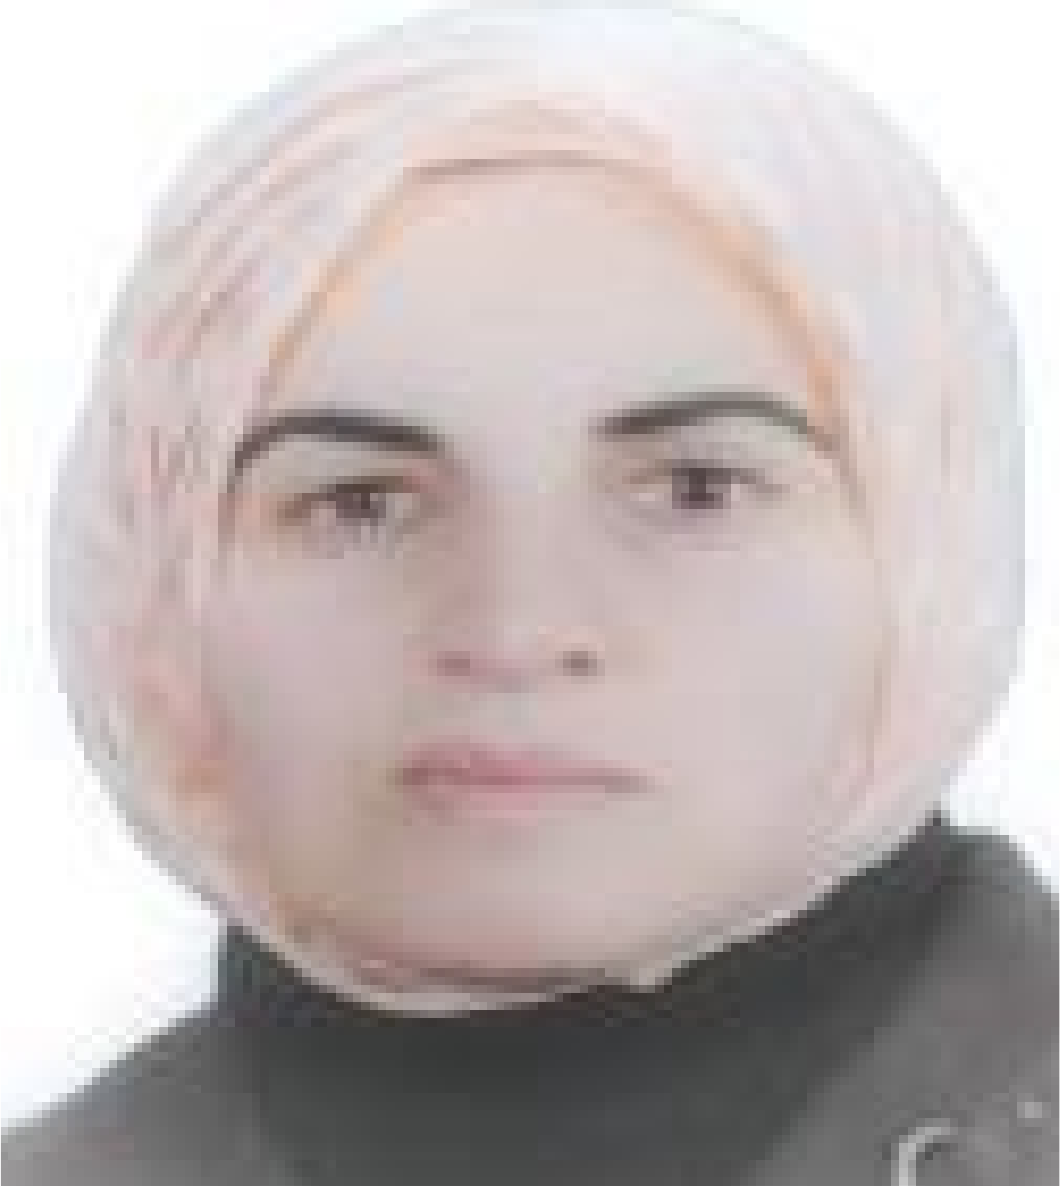
\includegraphics[width=1in,height=1.25in,clip,keepaspectratio]{abdulateef.png}}]{Salwa Khalid Abdulateef} received the B.Sc. and M.Sc. degrees in computer science from the University of Basrah, Iraq. She is currently a Lecturer with the Department of Computer Science, Tikrit University, Iraq. Her research interests include artificial intelligence, optimization, computer vision, image processing, information hiding and machine learning. She can be contacted at khalid.salwa@tu.edu.iq.
\end{IEEEbiography}

\EOD
\end{document}
